\documentclass[12pt, twoside]{article}
\title{Why a combination, $\Combination{n}{k}$, is always a natural number? Different way to look at the answer accentuates factors and prime numbers contained within a particular range of $1$ to $n$.}
\author{Amit Kumar}
\date{\today}
\usepackage[a4paper, margin=0.75in]{geometry}
\usepackage[page]{appendix}
\usepackage{amsmath}
\usepackage{amssymb}
\usepackage{mathtools}
\usepackage{xcolor}
\usepackage{ulem}
\usepackage{cancel}
\usepackage{listings}
\usepackage{pythonhighlight}
\usepackage{graphicx}
\usepackage{float}
\usepackage{url}
\newcommand*{\Permutation}[2]{{}^{#1}P_{#2}}%
\newcommand*{\Combination}[2]{{}^{#1}C_{#2}}%
\newcommand\bypassurl[1]{\textbf{URL:} \textit{#1}}
\begin{document}
	\maketitle
	\section{Abstract}
	 This article discusses why a combination $\Combination{n}{k}$ will always be a natural number and never a fraction or an irrational number. This article separates an $\Combination{n}{k}$ into selective, mutually exclusive and collectively exhaustive cases and then shows for each case that all the terms in a denominator have a corresponding multiple in the numerator. All $k$ for a particular $n$ for a $\Combination{n}{k}$ are visualized through plots to gain better understanding. This different way of looking at a Combination $\Combination{n}{k}$, gives hindsights into factors and prime numbers contained within a particular range of $1$ to $n$, in the context of the plots.
	\section{Introduction}
	From countless ages, it has been desired to know the number of ways an arrangement can be obtained or selected out of many possible ways. The quest has travelled from ancient times and has captured the imagination of the great mathematicians like Bhaskara-II, Blaise Pascal, Pierre-de-Fermat, Leonhard Euler to name a few.\newline	
	Permutations and Combinations have become fundamental concepts with wide ranging applications in almost every sphere of academic studies or technical endeavors.
	Combination, $\Combination{n}{k}$ represents number of ways $k$ elements out of $n$ can be choosen, \textit{without any regard to order between the choosen items}. It is defined as $\Combination{n}{k} = \frac{n!}{(n-k)!\times(k)!}$. While it is possible to show that each of the denominator terms $(n-k)!$ and $k!$ individually cancel terms in the numerator, it is not rigorously shown if the product of these two terms ever compete for a single numerator. If this condition is true where two terms in the denominator have a single term in the numerator, then the result will be a fraction and not a natural number. The results have indeed been observed to be integers empirically. However, surprisingly, a rigorous mathematical discussion on this question is relatively scarce. Some indirect proofs are definitely there such as using Pascal's triangle. The $n$'th  row of the Pascal's triangle is expansion of Binomial Coefficients, where each Coefficient is a combination ($\Combination{n}{k}$). It should be apparent that a rigorous proof of the observation that a combination will never be a fraction is crucial since many fundamental science concepts depend on it.\newline
	This paper aims to fill the gap and demonstrate that the final value of a combination will always collapse to an integer (more correctly a natural number). At the end of it we visualize our results and we find interesting connection of factors and prime numbers contained within the range $1$ to $n$ for a combination $\Combination{n}{1}$.
	\section{Methods}
	\subsection{Why permutation $\Permutation{n}{k}$ is a natural number?}
	Permutation is number of arrangements, when the order matters and is given by:\newline
	\begin{equation}
		\Permutation{n}{k} = \frac{n!}{(n-k)!}  \; \text{where n,k} \in \mathbb{N}  \; \text{and} \; 1 \leq k \leq n
	\end{equation}
	 e.g. Number of possibilities to choose $5$ items out of $9$ choices, we will write as $\Permutation{9}{5} =\frac{9!}{(9-5)!}$\newline
	 It is easy to show that $n!$ can be broken into multiplication two parts: one going from $n$ to $(n-k+1)$ and other going from $(n-k)$ to $1$. The denominator can also be written as multiplication of numbers from $(n-k)$ to $1$ as below.\newline
	 \begin{align*}
	 	\Permutation{n}{k} &= \frac{n!}{(n-k)!}\\
	 	&= \frac{(n)\times(n-1)\cdots\times(n-k+1)\times\color{red}(n-k)\times(n-k-1)\cdots\times3\times2\times1}{\color{red}(n-k)\times(n-k-1)\times(n-k-2)\cdots\times3\times2\times1}\\
	 	&= (n)\times(n-1)\cdots\times(n-k+1)
	 \end{align*}
 	Since each participating number in the product is a natural number, the net product is also a natural number.$\blacksquare$\newline
 	\subsection{Why Combination $\Combination{n}{k}$ is a natural number?}
 	Permutation is number of arrangements, when the order \textit{does not} matter and is given by:\newline
 	\begin{equation}
 		\Combination{n}{k} = \frac{n!}{(n-k)!\times(k)!} \; \text{where n,k} \in \mathbb{N} \; \text{and} \; 1 \leq k \leq n
 	\end{equation}
 	This time we can cancel the denominator's k!
 	\begin{align*}
 		\Combination{n}{k} &= \frac{(n)\times(n-1)\cdots\times(k+1)\times\color{red}(k)\times(k-1)\cdots\times3\times2\times1}{(n-k)\times(n-k-1)\cdots\times3\times2\times1\times\color{red}(k)\times(k-1)\cdots\times3\times2\times1}\\
 		&= \frac{(n)\times(n-1)\cdots\times(k+1)}{(n-k)\times(n-k-1)\cdots\times3\times2\times1}
 	\end{align*}
 Thus it can be written down as:
 \begin{equation}
 	\Combination{n}{k} = \frac{(k+1)\times(k+2)\cdots\times(n-1)\times(n)}{(n-k)\times(n-k-1)\cdots\times3\times2\times1} \label{reducedCombinationForm}
 \end{equation}
\subsubsection{Different possible values of $n$ and $k$ w.r.t each other.}
 If $n//2$ is defined as integer portion of division of $n$ by $2$, then we can see that one of the two below must be true:
 \begin{align}
 	n &= (n//2 \times 2) \; \text{where $n$ is an even number} \label{nIsEven}\\
 	n &= (n//2 \times 2) + 1 \; \text{where $n$ is an odd number} \label{nIsOdd}
 \end{align}
On a similar note, $k$ can be defined as six and six only possibilities w.r.t $n$:
\begin{align}
	k &= n//2 \; \text{where $n$ is an even number }\label{kEqualsCase1}\\
	k &= n//2 - l \; \text{where $n$ is an even number and } l \in \mathbb{N} , 1 \leq l \leq n//2 \label{kEqualsCase2}\\
	k &= n//2 + m \; \text{where $n$ is an even number and } m \in \mathbb{N} , 1 \leq m \leq n//2 \label{kEqualsCase3}\\
	k &= n//2 \; \text{where $n$ is an odd number }\label{kEqualsCase4}\\
	k &= n//2 - l \; \text{where $n$ is an odd number and } l \in \mathbb{N} , 1 \leq l \leq (n-1)/2 \label{kEqualsCase5}\\
	k &= n//2 + m \; \text{where $n$ is an odd number and } m \in \mathbb{N} , 1 \leq m \leq (n+1)/2) \label{kEqualsCase6}		
\end{align}
Let us take concrete examples to understand equations from \eqref{nIsEven} to \eqref{kEqualsCase6}.\newline\newline
$\Combination{10}{0}$ means $n$ is even, $k = 0$ and $l=n//2=5$: Thus equations \eqref{nIsEven} and \eqref{kEqualsCase2} are realized.\newline
$\Combination{10}{2}$ means n is even, $k = 2$ and $l=3$: Thus equations \eqref{nIsEven} and \eqref{kEqualsCase2} are realized.\newline
$\Combination{10}{4}$ means $n$ is even, $k = 4$ and $l=1$: Thus equations \eqref{nIsEven} and \eqref{kEqualsCase2} are realized.\newline\newline
$\Combination{10}{5}$ means $n$ is even and $k = n//2 = 5$: Thus equations \eqref{nIsEven} and \eqref{kEqualsCase1} are realized.\newline\newline
$\Combination{10}{6}$ means $n$ is even, $k = 6$ and $m=1$: Thus equations \eqref{nIsEven} and \eqref{kEqualsCase3} are realized.\newline
$\Combination{10}{8}$ means $n$ is even, $k = 8$ and $m=3$: Thus equations \eqref{nIsEven} and \eqref{kEqualsCase3} are realized.\newline
$\Combination{10}{10}$ means $n$ is even, $k = 10$ and $m= n//2=5$: Thus equations \eqref{nIsEven} and \eqref{kEqualsCase3} are realized.\newline\newline
$\Combination{11}{0}$ means $n$ is odd, $k = 0$ and $l=(n-1)/2=5$: Thus equations \eqref{nIsOdd} and \eqref{kEqualsCase5} are realized.\newline
$\Combination{11}{2}$ means n is odd, $k = 2$ and $l=3$: Thus equations \eqref{nIsOdd} and \eqref{kEqualsCase5} are realized.\newline
$\Combination{11}{4}$ means $n$ is odd, $k = 4$ and $l=1$: Thus equations \eqref{nIsOdd} and \eqref{kEqualsCase5} are realized.\newline\newline
$\Combination{11}{5}$ means $n$ is odd and $k = n//2 = 5$: Thus equations \eqref{nIsOdd} and \eqref{kEqualsCase4} are realized.\newline\newline
$\Combination{11}{6}$ means $n$ is odd, $k = 6$ and $m=1$: Thus equations \eqref{nIsOdd} and \eqref{kEqualsCase6} are realized.\newline
$\Combination{11}{8}$ means $n$ is odd, $k = 8$ and $m=3$: Thus equations \eqref{nIsOdd} and \eqref{kEqualsCase6} are realized.\newline
$\Combination{11}{11}$ means $n$ is odd, $k = 11$ and $m= (n+1)/2=6$: Thus equations \eqref{nIsOdd} and \eqref{kEqualsCase6} are realized.\newline\newline
We can clearly see based on equations \eqref{kEqualsCase1} to \eqref{kEqualsCase6} that there are six possibilities that we separately need to take care and prove. In the following subsections, \ref{ProofkEqualsCase1} to \ref{ProofkEqualsCase6}, we will prove each of the above condition.
\subsubsection{Setting up the problem}\label{settingUpTheProblem}
Looking at equation \eqref{reducedCombinationForm} it is clear that each term in the denominator can be written as $(n-k-x)$, where $x \in \mathbb{W}, 0 \leq x \leq (n-k-1)$ and each term in the numerator can be written as $(k+y)$, where $y \in \mathbb{N}, 1 \leq y \leq (n-k)$. Formalizing in equations as below:
\begin{align}
	\text{denominator} &= \prod_{0}^{n-k-1}(n-k-x), \text{where $n$ and $k$ are constants and $x$ is the variable} \label{denominator}\\
	\text{numerator} &= \prod_{1}^{n-k}(k+y), \text{where $k$ is a constant and $y$ is the variable} \label{numerator}
\end{align}
Now we have to show that for every $(n-k-x) \text{and } (k+y)$, there exists a natual number \textbf{$a$} such that $a \times (n-k-x) = (k+y)$ holds true. i.e.
\begin{equation}
	a \times (n-k-x) = (k+y), \text{where $a \in \mathbb{N}$}  \label{MultipleOfAisAnswer}
\end{equation}
\subsubsection{$\Combination{n}{k}$ is always a natural number when equation \eqref{nIsEven} and \eqref{kEqualsCase1} hold true}\label{ProofkEqualsCase1}
\begin{align}
	a \times (n-k-x) &= (k+y) \nonumber \\
	a \times (2\times n//2 - n//2 -x) &= (n//2+y) \nonumber \\
	a \times(n//2 -x) &= (n//2 + y) \nonumber \\
	a &= \frac{(n//2+y)}{(n//2-x)} \nonumber\\
	y &= a\times(n//2-x) - n//2 \nonumber \\
	y &= (a-1)\times n//2 - a\times x \label{yEqualsCase1}
\end{align}
Let us take a couple of examples. \newline
For $\Combination{10}{5} \text{ and } x = 1$ we get the solution as below
\begin{align*}
	y &= (a-1)\times 5 - a \\
	y &= a \times (5 - 1) - 5 \\
	y &= a \times 4 - 5 \\
\end{align*}
Clearly if $a = 2$ we get a valid solution and $y=3$. Let us see what this means. This means that for denominator $(n-k-x) = (10-5-1) = 4$, we will get a corresponding numerator which will have its factor as $(k+y) = (5+3) = 8$. This is consistent. Let us take another example.\newline
For $\Combination{10}{5} \text{ and } x = 3$ we get the solution as below
\begin{align*}
	y &= (a-1)\times 5 - a \times 3 \\
	y &= a \times (5 - 3) - 5 \\
	y &= a \times 2 - 5 \\
\end{align*}
Clearly if $a = 3$ we get a valid solution and $y=1$. Let us see what this means. This means that for denominator $(n-k-x) = (10-5-3) = 2$, we will get a corresponding numerator which will have its factor as $(k+y) = (5+1) = 6$. This is also consistent.\newline
For \eqref{yEqualsCase1}, we know that $x \in \mathbb{W}, 0 \leq x \leq (n-k-1)$ and $y \in \mathbb{N}, 1 \leq y \leq (n-k)$. These two conditions get simplified due to \eqref{kEqualsCase1} as $0 \leq x \leq (n//2-1)$. Let us put extreme conditions of $x$ to see if we can obtain a valid \textbf{$a$} for the denominator for every $y$.
\begin{align*}
	y &= (a-1)\times n//2 - a\times 0 \text{ this is due to \eqref{yEqualsCase1}} \\
	y &= (a-1)\times n//2
\end{align*}
Clearly an a can be choosen such that R.H.S is a natural number. Similarly we can say that,
\begin{align*}
	y &= (a-1)\times n//2 - a\times (n//2-1) \text{ this is due to \eqref{yEqualsCase1}} \\
	y &= \cancel{a\times n//2} - n//2 -\cancel{a\times n//2} +a \\	
	y &= a - n//2
\end{align*}
Clearly an \textbf{$a$} can be choosen such that R.H.S is a natural number. Thus we saw that an $a$ is available in the range of extreme $x$ values so that we always have \textbf{$a$} so that every denominator is a factor for some numerator.$\blacksquare$
\subsubsection{$\Combination{n}{k}$ is always a natural number when equation \eqref{nIsEven} and \eqref{kEqualsCase2} hold true}\label{ProofkEqualsCase2}
\begin{align}
	a \times (n-k-x) &= (k+y) \nonumber \\
	a \times (2\times n//2 - n//2 + l - x) &= (n//2 - l + y) \nonumber \\
	a &= \frac{(n//2 - l + y)}{(n//2 + l - x)} \nonumber \\
	y &= (a-1)\times n//2 + l \times (a+1) - a\times x \label{yEqualsCase2}	
\end{align}
How do we interpret this? Let us see an example. \newline
$\Combination{10}{4}$. Here $n = 10$ and thus $n//2 = 5, k = 4, l = n//2 - k = 5 -4 = 1$. Furthermore let us assume that $x = 1$, i.e. the denominator is $(n-k-1)$ for which the factor containing numerator has to be found.\newline
Putting the above values in \eqref{yEqualsCase2}, we get
$y = (a-1)5+1(a+1)-a\times 1 = (a-1)5+1$\newline
Clearly $a = 2$ will solve the equation which is consistent with restrictions on $y$ and the value of $y$ will be $y=(2-1)\times5 + 1=6$. That means the corresponding multiples will reside in the numerator $(k+y)=(k+6)$.\newline
Clearly, putting all the values in equation \eqref{MultipleOfAisAnswer} should get us no contradiction.
\begin{align}
	a \times (n-k-x) &= (k+y) \nonumber \\
	2 \times (10-4-1) &= (4+6) \nonumber \\
	2 \times (5) &= (10) \nonumber \\
	10 &= 10 \nonumber
\end{align}
Please note that $a = 1$ will also give a consistent solution as $y=(1-1)\times5 + 1=1$, which means $(k+1)$ as the numerator. It can be seen that $(n-k-x)=(10-4-1)=5$ will have two numerators where the multiples reside, one in $(k+1)=5$ and other in $(k+6)=10$.
Let us take another example as $\Combination{10}{4}$ and $x = 3$. i.e. the denominator is $(n-k-3)$ and the corresponding numerator, $(k+y)$, has to be found. Using \eqref{yEqualsCase2}, we get $y = (a-1)5+1(a+1)-a*3 = (a-1)5+6$\newline. Again $a=3$ will solve the equation and $y$ will be $y=(3-1)\times5 +1+ 3*3=2$. That means the corresponding factor will reside in the numerator $(k+y)=(k+2)$.\newline. To see if it is consistent, we will have to put the values in \eqref{MultipleOfAisAnswer}.
\begin{align}
	a \times (n-k-x) &= (k+y) \nonumber \\
	2 \times (10-4-3) &= (4+2) \nonumber \\
	2 \times (3) &= (6) \nonumber \\
	6 &= 6 \nonumber
\end{align}
Now according to \eqref{denominator}, 
\begin{align}
	0 \leq x \leq (n-k-1) &= 0 \leq x \leq (2\times n//2-n//2+l-1) \nonumber \\
	&= 0 \leq x \leq (n//2+l-1) \label{LimitOfXforYEqualsCase2}
\end{align}
We will show that the equations are consistent at the extremes of $x$ and therefore must be true for other values of $x$.\newline
Choosing $x=0$ in the equation \eqref{yEqualsCase2}, we get
\begin{align*}
	y &= (a-1)\times n//2 + l \times (a+1) - a\times x \\
	y &= (a-1)\times n//2 + l \times (a+1) - a\times 0 \\
	y &= (a-1)\times n//2 + l \times (a+1)
\end{align*}
Since $l$ is $a \in \mathbb{N}$, so the minimum value $l$ can have is $1$. Thus the second term in the R.H.S. above will be positive. To make $y$ as positive integer, there is always a value of $a$ we can choose to satisfy this restriction.\newline
At the other extreme, choosing $x=(n//2+l-1)$, we get the below.
\begin{align*}
	y &= (a-1)\times n//2 + l \times (a+1) - a\times (n//2+l-1) \\
	y &= a\times n//2 - n//2 +l\times a +l -a\times n//2-a\times\ l + a \\
	y &= \cancel{a\times n//2} - n//2 +\cancel{l\times a} +l -\cancel{a\times n//2}-\cancel{a\times\ l} + a \\
	y &= a - n//2 + l 
\end{align*}
Again it is evident that an $a$ can be choosen such that $y$ can be in a form consistent with assumptions. Thus we have shown that the equation \eqref{yEqualsCase2} is consistent and solvable at extremes of $x$ and thus must be solvable between. $\blacksquare$
\subsubsection{$\Combination{n}{k}$ is always a natural number when equation \eqref{nIsEven} and \eqref{kEqualsCase3} hold true}\label{ProofkEqualsCase3}
\begin{align}
	a \times (n-k-x) &= (k+y) \nonumber \\
	a \times (2\times n//2 - n//2 - m - x) &= (n//2 + m + y) \nonumber \\
	a &= \frac{(n//2 +m + y)}{(n//2 -m - x)} \nonumber \\
	y &= (a-1)\times n//2 - m \times (a+1) - a\times x \label{yEqualsCase3}	
\end{align}
Interpreting this result is as before through an example.\newline
$\Combination{10}{6}$. Here $n = 10$ and thus $n//2 = 5, k = 6, m = k - n//2 = 6 - 5 = 1$. Furthermore let us assume that $x = 1$, i.e. the denominator is $(n-k-1)$ for which the factor containing numerator has to be found.\newline.
Substituting the above values in \eqref{yEqualsCase3}, we get  $y = (a-1)5-m(a+1)-a*1 = (a-1)5-1(1+a)-a = (a-1)5-2a-1$\newline. 
It is easy to see that the equation is solved for $a = 3$. In such a case $y$ will be equal to $(3-1)*5-2*3-1 = 3$. i.e. for $(n-k-1)$, there is a multiple in $(k+3)$, where $n=10$ and $k=6$. It is trivial to verify this.
\begin{align*}
	a \times (n-k-x) &= (k+y) \\
	3 \times (10-6-1) &= (6+3) \\
	3 \times (3) &= (9) \\
	9 &= 9 
\end{align*}
As per \eqref{denominator}, 
\begin{align}
	0 \leq x \leq (n-k-1) &= 0 \leq x \leq (2\times n//2-n//2-m-1) \nonumber \\
	&= 0 \leq x \leq (n//2-m-1) \label{LimitOfXforYEqualsCase3}
\end{align}
We need to show that there is no contradiction at the extremes \eqref{yEqualsCase3} and thus it will hold true for middle values as well.
Choosing $x = 0$ in equation \eqref{yEqualsCase3} we arrive at,
\begin{align*}
	y &= (a-1)\times n//2 - m \times (a+1) - a\times x \\
	y &= (a-1)\times n//2 - m \times (a+1) - a\times 0 \\
	y &= (a-1)\times n//2 - m \times (a+1)
\end{align*}
 The above should hold for $y \geq 1$. Thus
 \begin{align*}
 	(a-1)\times n//2 \geq 1 +  m \times (a+1) \\
 	a\times n//2 -m\times a \geq (1+m+n//2) \\
 	a \geq \frac{(1+m+n//2)}{(n//2-m)}
 \end{align*}
The last equation is defined as long as $n//2 \ge m$. This constraint is already in place due to the premise of \eqref{kEqualsCase3}. Thus a value of \textbf{$a$} can be computed such that \eqref{yEqualsCase3} is satisfied.\newline
Working at the other extreme of $x = (n//2 - m -1)$ we observe the below.
\begin{align*}
	y &= (a-1)\times n//2 -m \times(1+a) -a \times (n//2 -m -1) \\
	y &= a\times n//2 - n//2 -m -m\times a -a \times n//2 - a\times m + a \\
	y &= \cancel{a\times n//2} - n//2 -m -\cancel{m\times a} -\cancel{a \times n//2} - \cancel{a\times m} + a \\
	y &= (a - n//2) - m
\end{align*}
As seen, $y$ has allowed solutions at both extremes as there is always an a that can be choosen to satisfy the constraints.$\blacksquare$
\subsubsection{$\Combination{n}{k}$ is always a natural number when equation \eqref{nIsOdd} and \eqref{kEqualsCase4} hold true}\label{ProofkEqualsCase4}
\begin{align}
	a \times (n-k-x) &= (k+y) \nonumber \\
	a \times (2\times n//2 + 1 - n//2 - x) &= (n//2 + y) \nonumber \\
	a &= \frac{(n//2 + y)}{(n//2 + 1 - x)} \nonumber \\
	y &= (a-1)\times n//2 + a - a\times x \label{yEqualsCase4}	
\end{align}
The best way to understand the above equation, as before, is through an example.\newline
In $\Combination{11}{5}$, $n=11$, $n//2=5=k$. Let $x$ be equal to $1$, then substituting the values in the above equation, we get,
\begin{align*}
	y = (a-1)\times 5 + a - a\times 1 \\
	y = (a-1)\times 5 + \cancel{a} - \cancel{a\times 1} \\
	y = (a-1)\times 5
\end{align*}
Clearly $a = 2$ will give a solution and $y$ will be equal to $5$. That means for the above setup for $(n-k-1)$, there will be a factor in $(k+5)$. It is easy to verify this.\newline
\begin{align*}
	a \times (n-k-x) &= (k+y) \nonumber \\
	2 \times (11-5-1) &= (5+5) \nonumber \\
	2 \times (5) &= (10) \nonumber \\
	10 &= 10
\end{align*}
Just like before we can appreciate that the equation \eqref{yEqualsCase4} has boundaries for extreme values of $x$. Thus if we show the lower extreme and upper extreme values of $x$ to have a consistent solution, then the proof must hold for values in between.\newline
We remember that $0 \leq x \leq (n-k-1)=0 \leq x \leq (2\times n//2 + 1-n//2-1)=0 \leq x \leq n//2$. First we will check for the lower limit of $0$. Putting $0$ in equation \eqref{yEqualsCase4}, we get,
\begin{align*}
	y &= (a-1)\times n//2 + a - a\times x \\
	y &= (a-1)\times n//2 + a - a\times 0 \\
	y &= (a-1)\times n//2 + a \\
\end{align*}
Clearly a value of $a$ can be choosen such that R.H.S satisfies the constraint that $y \in \mathbb{N}$. When we think of the other extreme, we obtain the following.
\begin{align*}
	y &= (a-1)\times n//2 + a - a\times x \\
	y &= (a-1)\times n//2 + a - a\times (n-k-1) \\
	y &= (a-1)\times n//2 + a - a\times (2\times n//2 + 1-n//2-1) \\
	y &= (a-1)\times n//2 + a - a\times (n//2) \\
	y &= a - n//2
\end{align*}
Here also it is clear that a value of \textbf{$a$} can be choosen such that the R.H.S is greater than or equal to $1$. \newline
Thus we have shown that a valid $y$ can be obtained by choosing an appropriate $a$, for two extreme values of $x$.$\blacksquare$
\subsubsection{$\Combination{n}{k}$ is always a natural number when equation \eqref{nIsOdd} and \eqref{kEqualsCase5} hold true}\label{ProofkEqualsCase5}
\begin{align}
	a \times (n-k-x) &= (k+y) \nonumber \\
	a \times (2\times n//2 + 1 - n//2 +l - x) &= (n//2 -l + y) \nonumber \\
	a &= \frac{(n//2 -l + y)}{(n//2 + 1 +l - x)} \nonumber \\
	y &= (a-1)\times n//2 + l\times(a+1) - a\times x + a \label{yEqualsCase5}	
\end{align}
Let us find the value for an example. Suppose we are given $\Combination{11}{4}$. Here $n=11$, $n//2=5$, $k=4$, $l=1$ and let's say $x=1$. Then putting these values in the above equation, we get:
\begin{align*}
	y &= (a-1)\times n//2 + l\times(a+1) - a\times x + a \\
	y &= (a-1)\times 5 + 1\times(a+1) - a\times 1 + a \\
	y &= (a-1)\times 5 + \cancel{1\times a}+ 1 - \cancel{a\times 1} + a \\
	y &= (a-1)\times 5 + 1 + a \\
\end{align*}
Clearly $a=1$ gives a solution and thus $y=2$. This argues that for $(n-k-1)$, there is a factor in $(k+2)$ for this example. i.e. for $(11-4-1)$ we have a factor in $(4+2)$. It is evident that $6$ is on both sides of the equation.\newline
Now we have to show that given an $x$ and $l$ and $n$, we can get a $y$ such that $y \in \mathbb{N}$. We will show for two extreme values of $x$, it should hold true for values in between.\newline
Let's recall that $0 \leq x \leq (n-k-1) = 0 \leq x \leq (2\times n//2+1-n//2+l-1) = 0 \leq x \leq (n//2 + l)$. Starting with $x=0$ and substituting $x=0$ in equation \eqref{yEqualsCase5}.
\begin{align*}
	y &= (a-1)\times n//2 + l\times(a+1) - a\times x + a \\
	y &= (a-1)\times n//2 + l\times(a+1) - a\times 0 + a \\	
	y &= (a-1)\times n//2 + l\times(a+1) + a \\		
\end{align*}
In the above each term on the right hand side is a positive integer and therefore the net value of $y$ is also going to be a positive integer and thus the restriction that $1 \leq y, y \in \mathbb{N}$\newline
Putting the other extreme value of $x$ in equation \eqref{yEqualsCase5}
\begin{align*}
	y &= (a-1)\times n//2 + l\times(a+1) - a\times x + a \\
	y &= (a-1)\times n//2 + l\times(a+1) - a\times (n//2+l) + a \\	
	y &= a\times n//2 - n//2 - l\times a + l -a\times n//2 - a \times l + a \\
	y &= \cancel{a\times n//2} - n//2 - \cancel{l\times a} + l -\cancel{a\times n//2} - \cancel{a \times l} + a \\
	y &= a - n//2 + l \\
\end{align*}
Given the limits on $l$ as per equation \eqref{kEqualsCase5}, a value of $l$ can be found such that a consistent value of $y$ can be obtained. $\blacksquare$\\
\subsubsection{$\Combination{n}{k}$ is always a natural number when equation \eqref{nIsOdd} and \eqref{kEqualsCase6} hold true}\label{ProofkEqualsCase6}
\begin{align}
	a \times (n-k-x) &= (k+y) \nonumber \\
	a \times (2\times n//2 + 1 - n//2 -m - x) &= (n//2 +m + y) \nonumber \\
	a &= \frac{(n//2 +m  + y)}{(n//2 + 1 +-m - x)} \nonumber \\
	y &= (a-1)\times n//2 -m\times(a+1) - a\times x + a \label{yEqualsCase6}	
\end{align}
Let us see the equation \eqref{yEqualsCase6} in action. \newline
Suppose it is given that we have to work on $\Combination{11}{6}$, then $n=11,n//2=5,k=6,m=1$. Furthermore suppose $x=3$, i.e. we have to find the multiple of $(n-k-3)$ in the numerator.
\begin{align*}
	y &= (a-1)\times n//2 -m\times(a+1) - a\times x + a \\
	y &= (a-1)\times 5 - 1\times(a+1) - a\times 3 + a \\
	y &= (a-1)\times 5 -1 -3\times a \\
	y &= 5\times a - 5 -1 -3\times a \\
	y &= 2\times a - 6
\end{align*}
Clearly there is a solution for $a = 4$. Once we have obtained, a then we can plug it in equation \eqref{yEqualsCase6} to obtain the value of $y$. We get,
\begin{align*}
	y &= (a-1)\times n//2 -m\times(a+1) - a\times x + a \\
	y &= (4-1)\times 5 -1\times(4+1) - 4\times 3 + 4 \\
	y &= 15 - 5 -12 + 4 \\
	y &= 2
\end{align*}
Thus for $\Combination{11}{6}$, for the numerator $(n-k-3)$, there is a factor in $(k+2)$. It is easy to verify this using \eqref{MultipleOfAisAnswer}. Putting the values:
\begin{align*}
	4\times(11-6-3) &= (6+2)\\
	4\times 2 &= 8
\end{align*}
Thus we arrive at a consistent solution.\newline
What is left to be shown is that given an $x$, $m$ and $n$, we can always get a $y$ such that $y \in \mathbb{N}$. Since $x$ has limits in equation \eqref{yEqualsCase6}, it suffices to show that a consistent $y$ can be obtained always if consistent $y$ can be obtained at the lower and upper extremes.\newline
Now $0 \leq x \leq (n-k-1) = 0 \leq x \leq (2\times n//2+1-n//2-m-1) = 0 \leq x \leq (n//2 -m)$. Given this premise, we first substitute the lower limit of $x$ which is $0$.
\begin{align*}
	y &= (a-1)\times n//2 -m\times(a+1) - a\times x + a \\
	y &= (a-1)\times n//2 -m\times(a+1) - a\times 0 + a \\
	y &= (a-1)\times n//2 -m\times(a+1) + a \\
	y &= a\times(n//2-m+1) - (n//2+m) \\
\end{align*}
So as long as $a\times(n//2-m+1) - (n//2+m) \geq 1$, the RHS will be a natural number and consistent $y$ can be obtained.
\begin{align}
	a\times(n//2-m+1) - (n//2+m) &\geq 1 \nonumber \\
	a\times(n//2-m+1) &\geq (n//2+m+1) \nonumber \\
	a &\geq \frac{(n//2+m+1)}{(n//2-m+1)} \label{tempAforYequals6-1}
\end{align}
Thus for the above to hold true $(1+n//2-m) \geq 0$.\newline
Due to constraints imposed by \eqref{ProofkEqualsCase6} 
\begin{align*}
	m \leq (n+1)/2 \\
	m \leq (2\times n//2 + 1 +1)/2 \\
	m \leq (2\times n//2 + 2)/2 \\
	m \leq (n//2+1) \\
	0 \leq (1+n//2-m)
\end{align*}
So the requirement is already satisfied for \eqref{tempAforYequals6-1} and thus for $x=0$ it is always possible to have a $y \in \mathbb{N}$. Now let us see the other extreme of $x$ which is $(n//2-m)$. Putting this value in equation \eqref{yEqualsCase6}.
\begin{align*}
	y &= (a-1)\times n//2 -m\times(a+1) - a\times x + a \\
	y &= (a-1)\times n//2 -m\times(a+1) - a\times(n//2-m) + a\\
	y &= a\times n//2 -n//2 -m\times a - m -a\times n//2 +a\times m + a \\
	y &= \cancel{a\times n//2} -n//2 -\cancel{m\times a} - m -\cancel{a\times n//2} +\cancel{a\times m} + a \\
	y &= (a - n//2) -m 
\end{align*}
If $(a - n//2) -m \geq 1$, the RHS will always be a positive integer and a consistent $y$ can be obtained.
\begin{align}
	(a - n//2) -m  &\geq 1 \nonumber \\
	a &\geq (n//2+m+1) \label{tempAforYequals6-2}
\end{align}
Since the R.H.S is a positive integer it is always possible to get such a value of $a$ and thus $y$ can be obtained for the other extreme of $x$, as well.$\blacksquare$
\section{Conclusion}\label{Summary}
This article discusses about $\Combination{n}{k}$, where if $n$ is even it can be written as $2*n//2$ (where $n//2$ is the integer part of division of $n$ by $2$) while it can be stated as $2*n//2+1$ if it is odd. Furthermore $k$, can take only three values: $(n//2), (n//2 - l) \text{ or } (n//2 + m)$, where $l$ and $m$ are positive integers greater than $1$, and they denote \textit{less} and \textit{more} respectively.\newline\newline
The denominator is composed of product of $(n-k-x)$ terms, while the numerator is composed of products of $(k+y)$ terms, with the following constraints.\newline\newline
$0 \leq x \leq (n-k-1)$\newline
$1 \leq y \leq (n-k)$\newline

With these premises we obtain the following relationship table between $y$ and $x$ (given $n$ and $k$). Please note that $l$ and $m$ need not be supplied and can always be calculated if $n$ and $k$ are given. However $l$ and $m$ must be known/calculated before using any of the below equations. Also, in the below table, the equation must be solved for all possible values of $\textbf{$a$}$ using the following algorithm.
\begin{enumerate}
    \item Decide $n$ is even or odd.
    \item given $k$ and $n$, decide if $l$ or $m$ is there and if yes what value.
    \item Get range of $x$ such that $0 \leq x \leq (n-k-1)$
    \item Solve for all values of $a$ (for each $x$) using the below table such that $1 \leq y \leq (n-k)$.
    \item For each $a$ get a feasible and corresponding $y$.
\end{enumerate}
\begin{tabular}{|l ||l ||l|}
	\hline
	\textbf{$n$} & \textbf{$k$} & \textbf{$y$} \\
	\hline
	Even & $n//2 \pm 0$ \space(i.e. $k = n//2$) & $y = (a-1)\times n//2 - a\times x$ \\
	\hline
	Even & $n//2 - l$ \space(i.e. $k < n//2$) & $y = (a-1)\times n//2 + l \times (a+1) - a\times x$ \\
	\hline
	Even & $n//2 + m$ (i.e. $k > n//2$) & $y = (a-1)\times n//2 - m \times (a+1) - a\times x$ \\
	\hline
	Odd & $n//2 \pm 0$ \space(i.e. $k = n//2$) & $y = (a-1)\times n//2 + a - a\times x$ \\
	\hline
	Odd & $n//2 - l$ \space(i.e. $k < n//2$) & $y = (a-1)\times n//2 + a + l\times(a+1) - a\times x$ \\
	\hline
	Odd & $n//2 + m$ (i.e. $k > n//2$)  & $y = (a-1)\times n//2 + a -m\times(a+1) - a\times x$ \\
	\hline
\end{tabular}\newline\newline
There can be an equivalent table where all the $a$ terms are brought together. The below table can help find $a$ quicker since all other terms are known. We can keep increasing $a$ by $1$ so that $y$ stays in the range as per premise.\newline\newline
\begin{tabular}{|l ||l ||l|}
	\hline
	\textbf{$n$} & \textbf{$k$} & \textbf{$y$} \\
	\hline
	Even & $n//2$ \space(i.e. $k = n//2$) & $y = a \times (n//2-x) - n//2$ \\
	\hline
	Even & $n//2 - l$ \space(i.e. $k < n//2$) & $y = a \times (n//2-x+l ) - n//2 + l$ \\
	\hline
	Even & $n//2 + m $ (i.e. $k > n//2$) & $y = a \times (n//2-x-m ) - n//2 -m$ \\
	\hline
	Odd & $n//2 $ \space(i.e. $k = n//2$) & $y = a \times (n//2-x +1) - n//2$ \\
	\hline
	Odd & $n//2 - l $ \space(i.e. $k < n//2$) & $y = a \times (n//2-x+l +1) - n//2 + l$ \\
	\hline
	Odd & $n//2 + m $ (i.e. $k > n//2$)  & $y = a \times (n//2-x-m +1 ) - n//2 -m $ \\
	\hline
\end{tabular}
\subsection{Visualizing the relationship between x and y as in \ref{Summary}}
For \eqref{yEqualsCase1}, \eqref{yEqualsCase2}, \eqref{yEqualsCase3}, \eqref{yEqualsCase4}, \eqref{yEqualsCase5} and \eqref{yEqualsCase6}, we can have plots, where for each plot $x$ is on the abscissa while $y$ is on ordinate for different values of $\Combination{n}{k}$ (with implicit $l$ or $m$ if applicable).
\begin{figure}[ph!]
	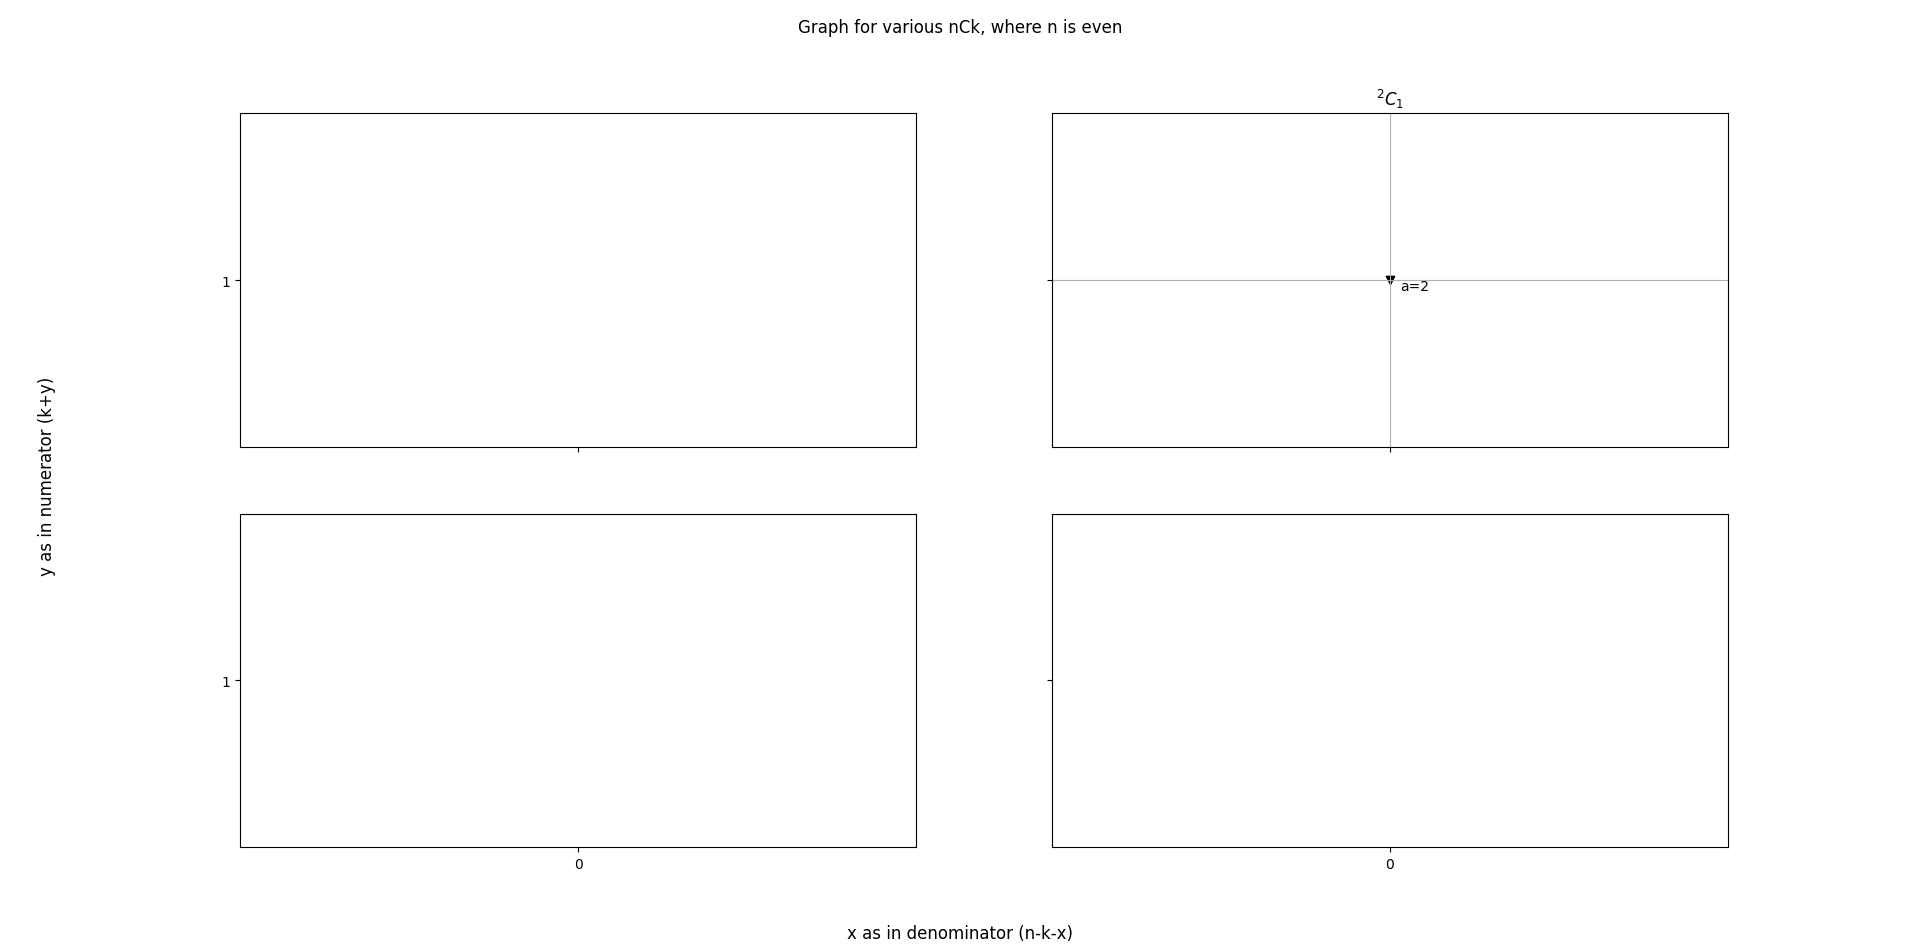
\includegraphics[width=\linewidth]{2Ck.png}
	\caption{Plot of $\Combination{2}{k}$}
	\label{2Ck}
\end{figure}
\begin{figure}[ph!]	
	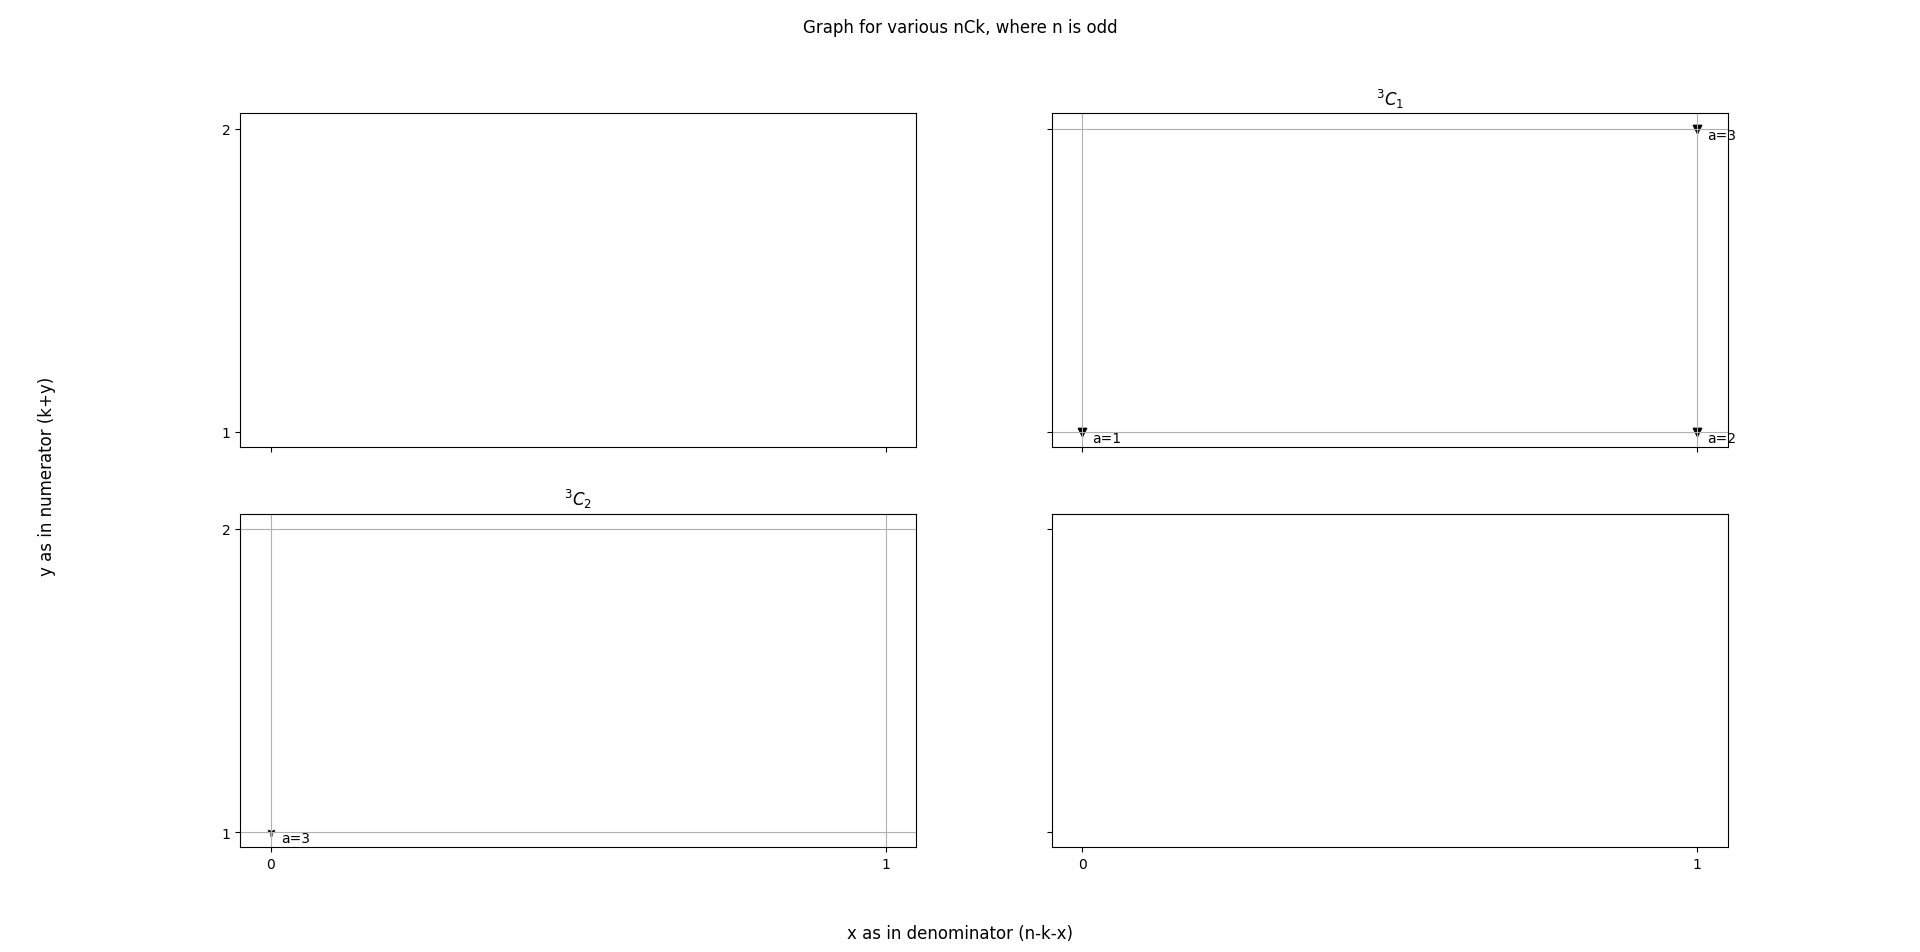
\includegraphics[width=\linewidth]{3Ck.png}
	\caption{Plot of $\Combination{3}{k}$}
	\label{3Ck}
\end{figure}
\begin{figure}[ph!]	
	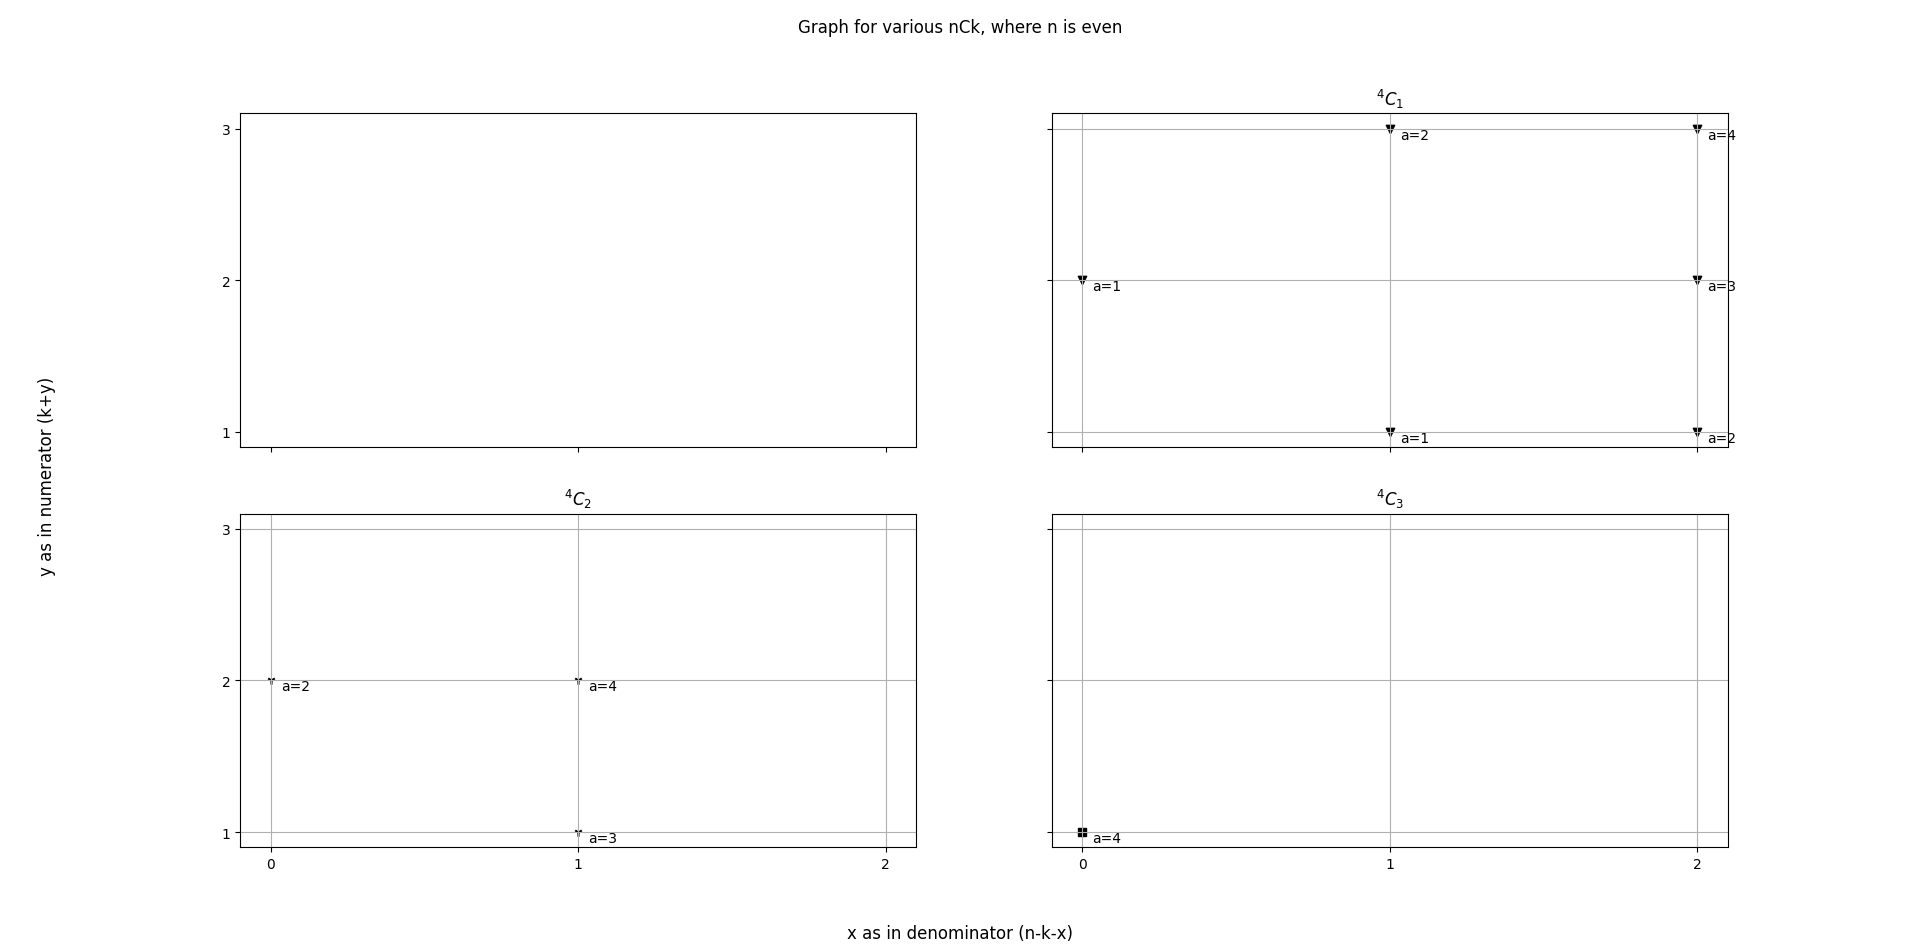
\includegraphics[width=\linewidth]{4Ck.png}
	\caption{Plot of $\Combination{4}{k}$}
	\label{4Ck}
\end{figure}
\begin{figure}[ph!]	
	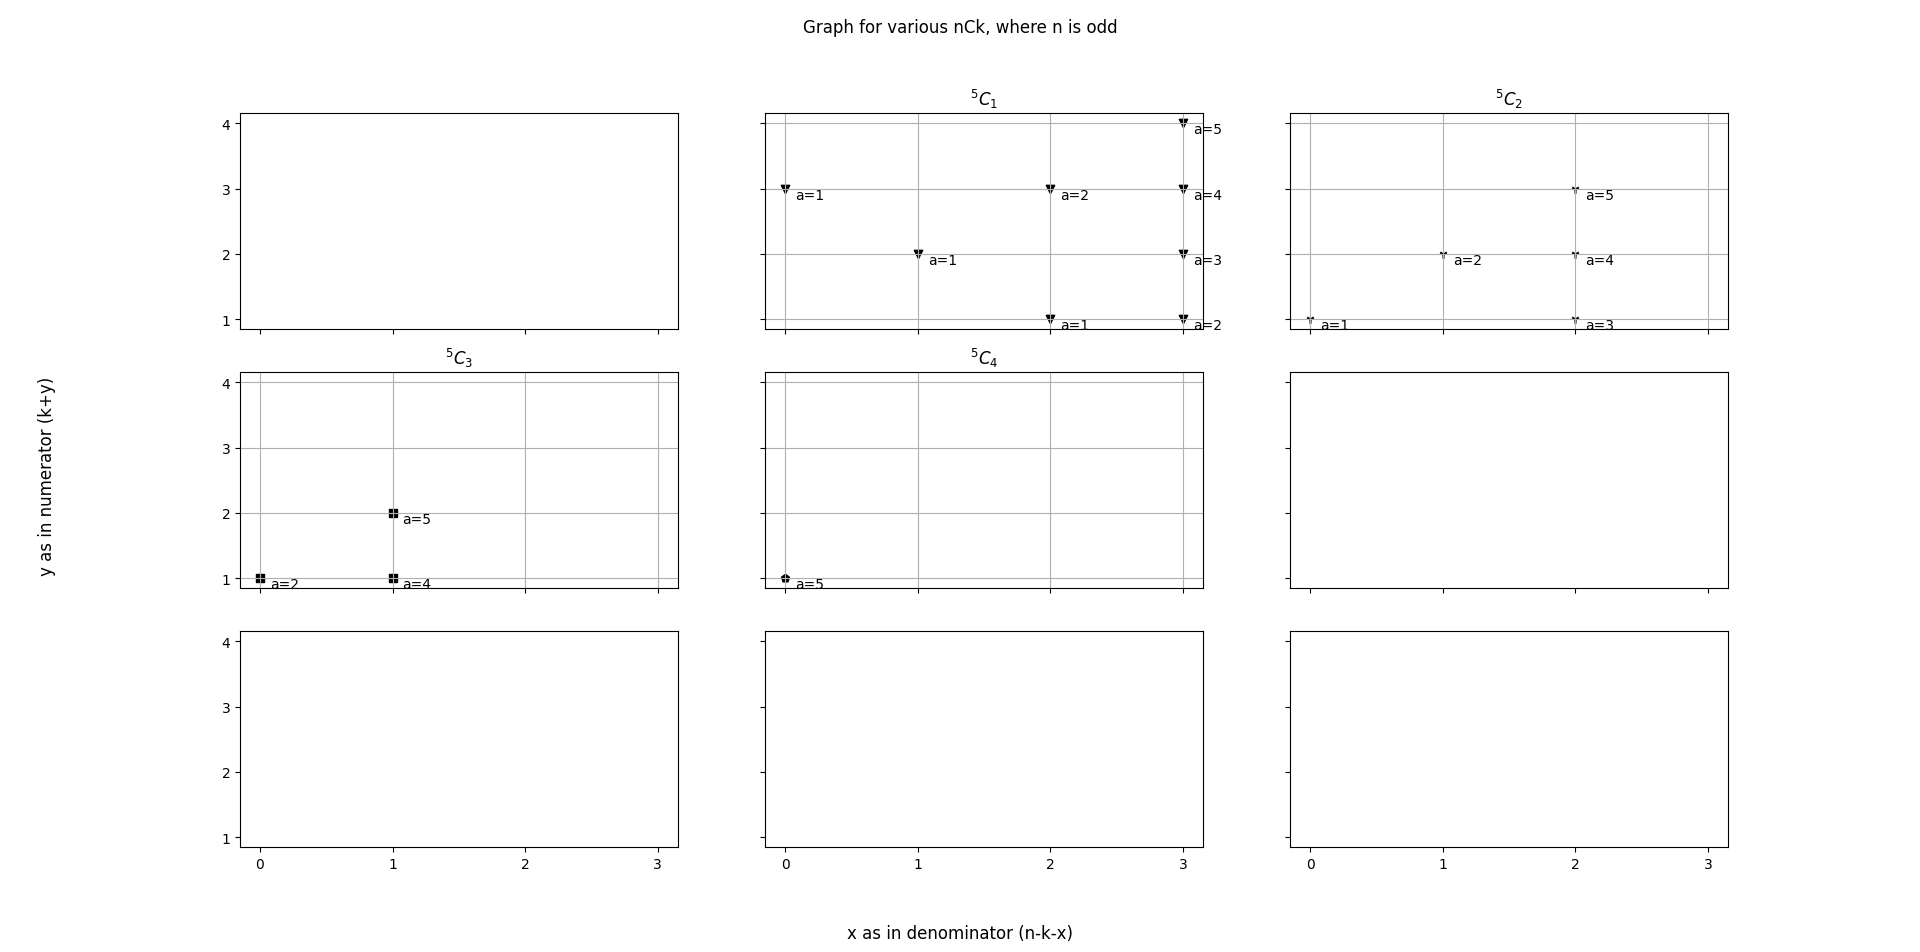
\includegraphics[width=\linewidth]{5Ck.png}
	\caption{Plot of $\Combination{5}{k}$}
	\label{5Ck}
\end{figure}
\begin{figure}[ph!]	
	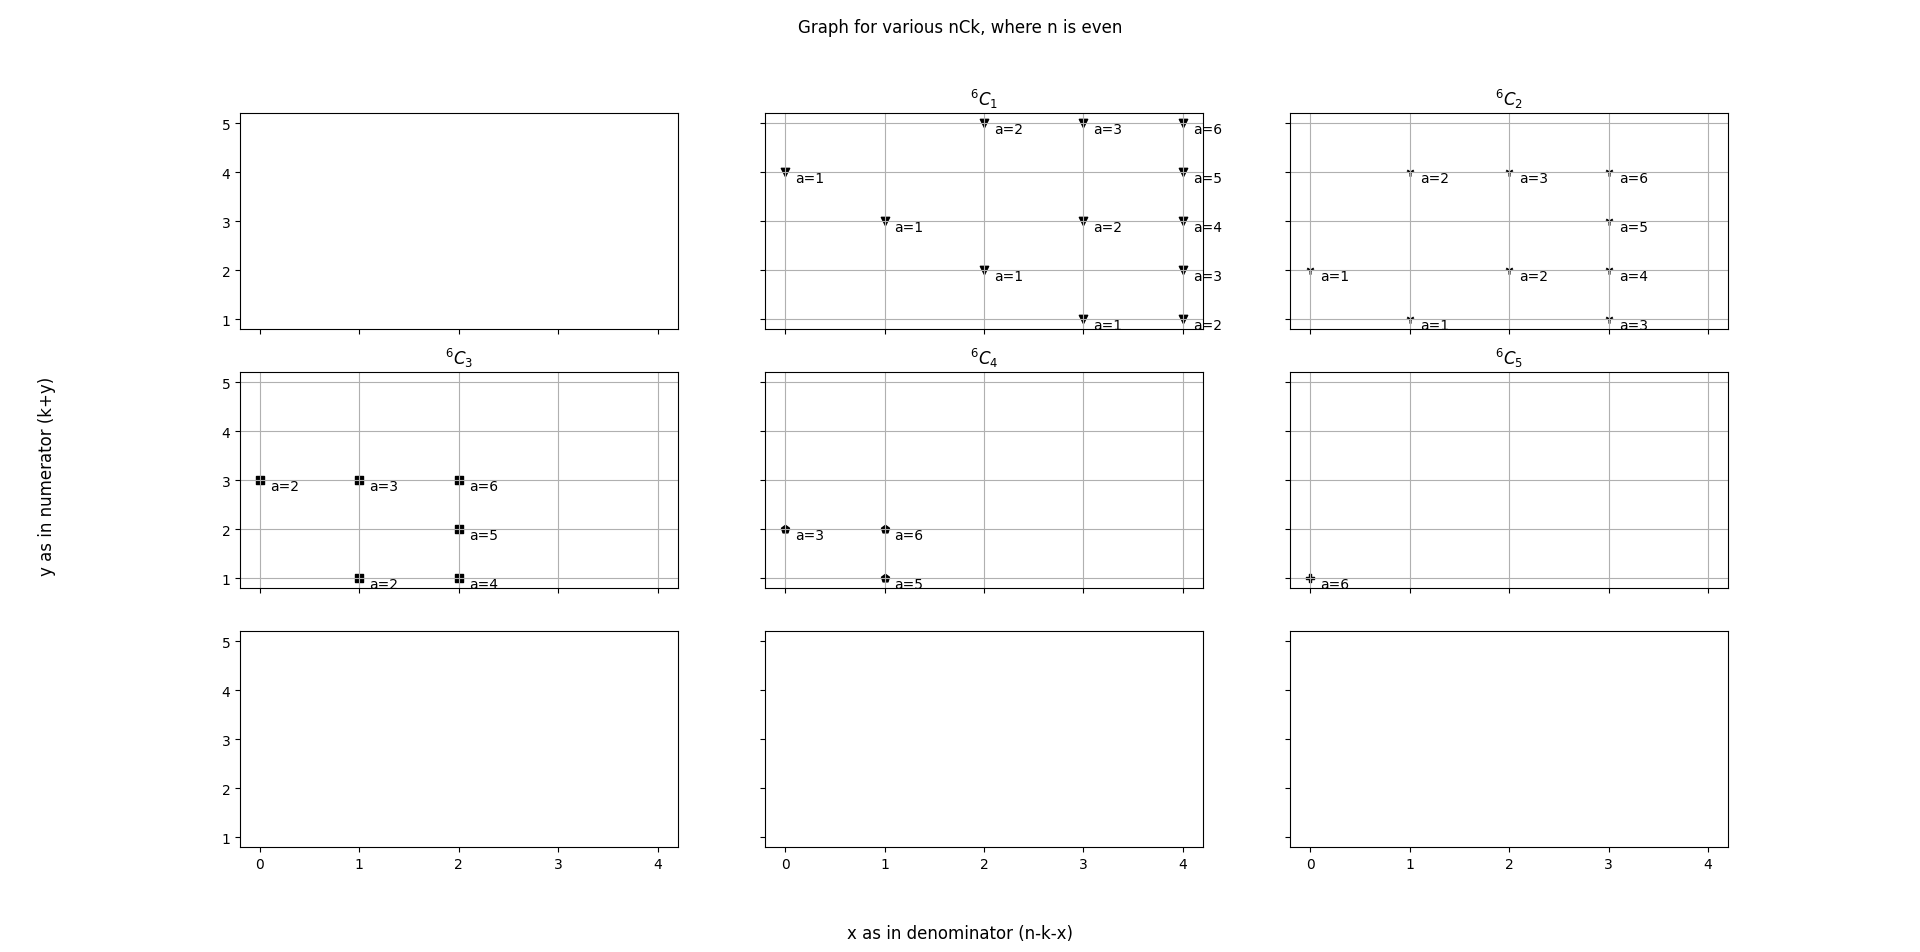
\includegraphics[width=\linewidth]{6Ck.png}
	\caption{Plot of $\Combination{6}{k}$}
	\label{6Ck}
\end{figure}
\begin{figure}[ph!]	
	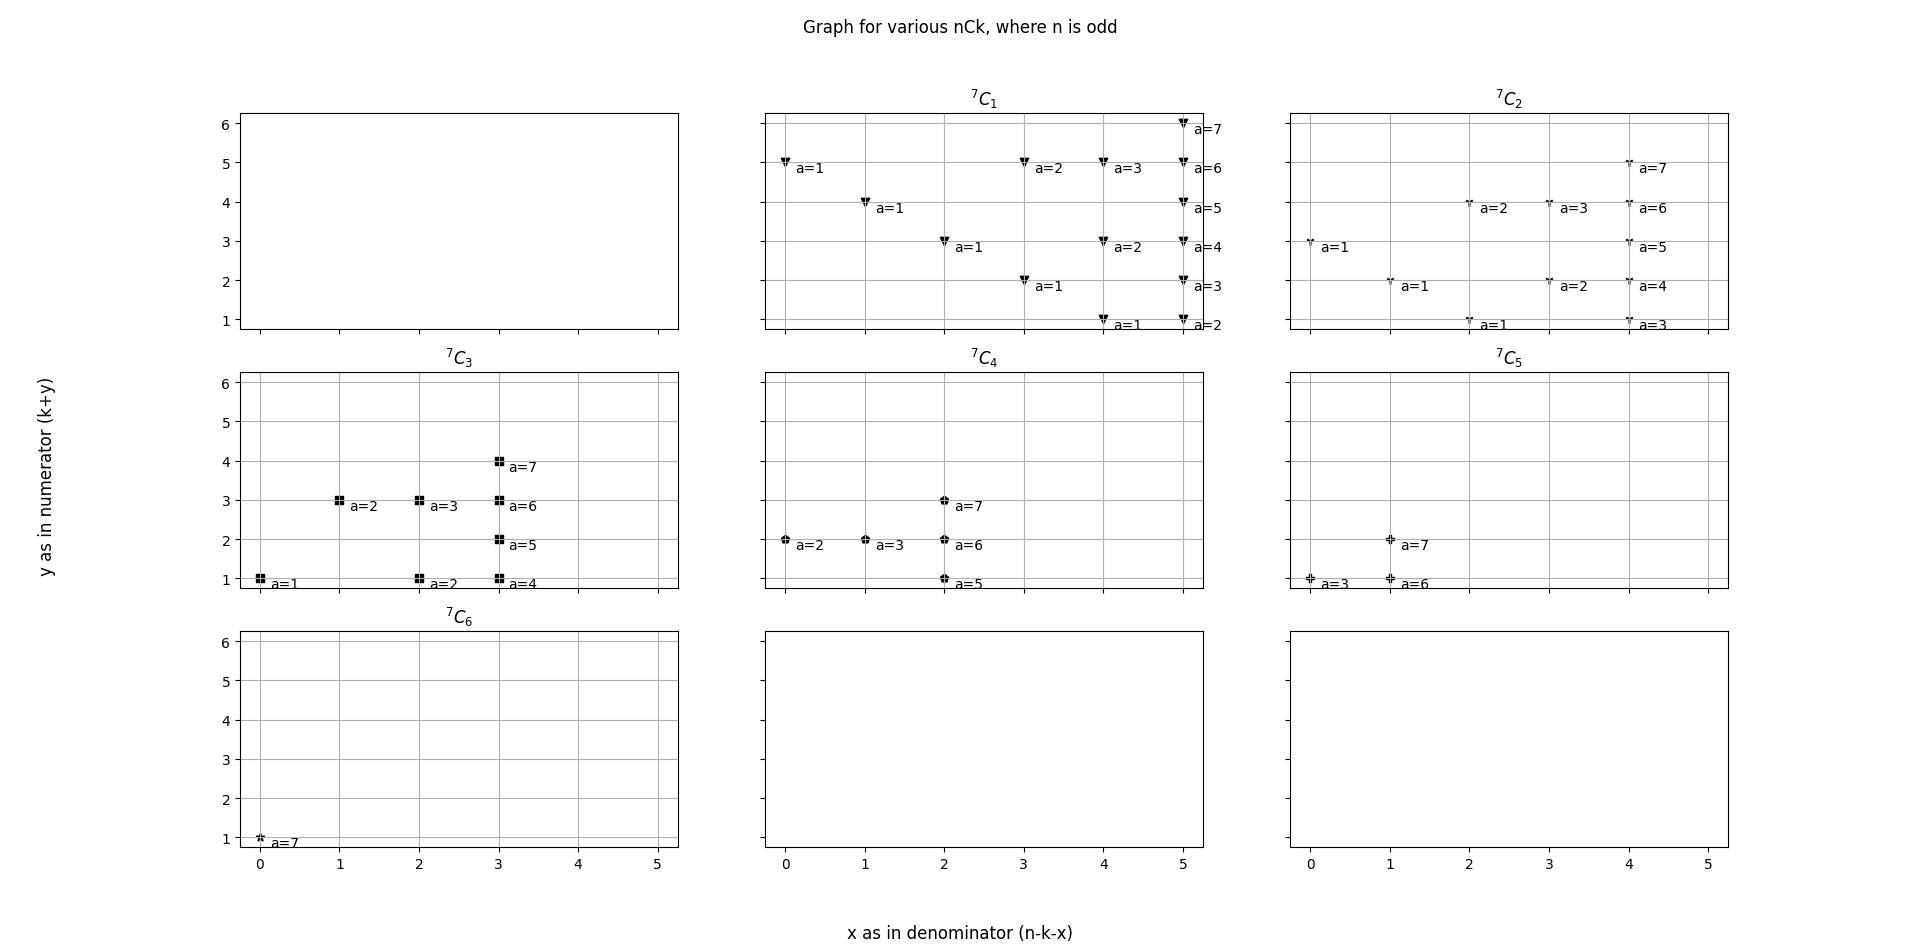
\includegraphics[width=\linewidth]{7Ck.png}
	\caption{Plot of $\Combination{7}{k}$}
	\label{7Ck}
\end{figure}
\begin{figure}[ph!]	
	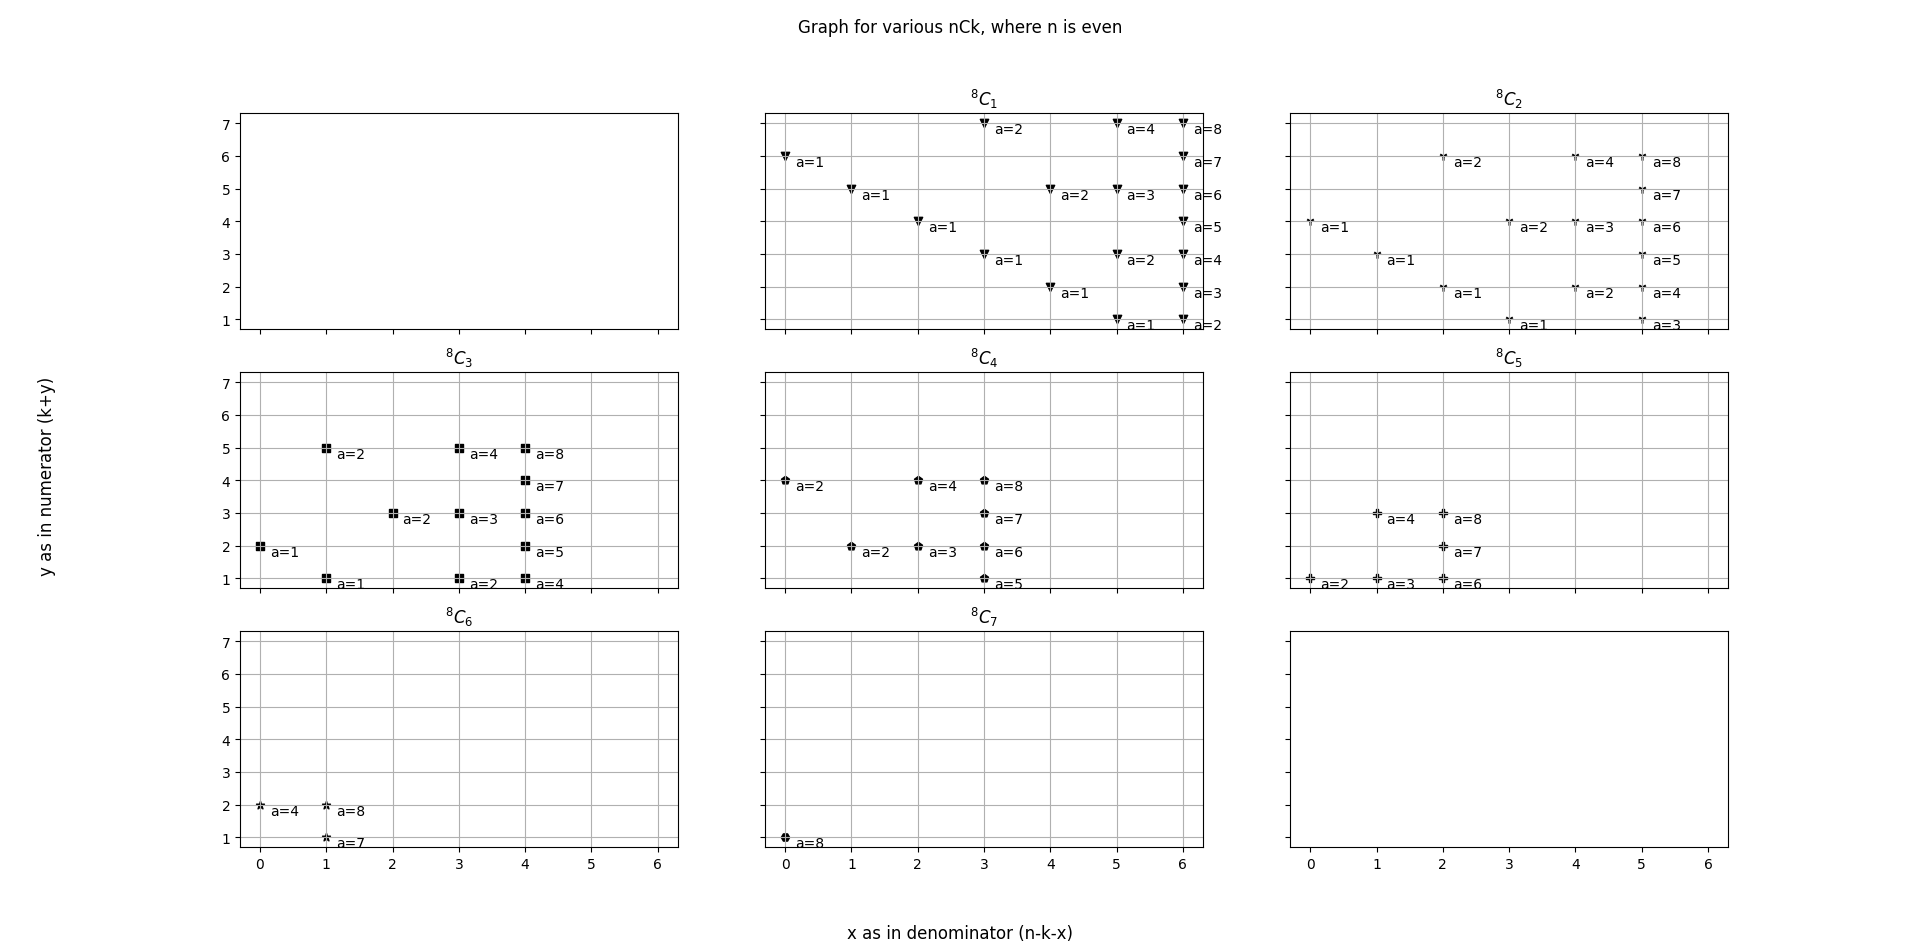
\includegraphics[width=\linewidth]{8Ck.png}
	\caption{Plot of $\Combination{8}{k}$}
	\label{8Ck}
\end{figure}
\begin{figure}[ph!]	
	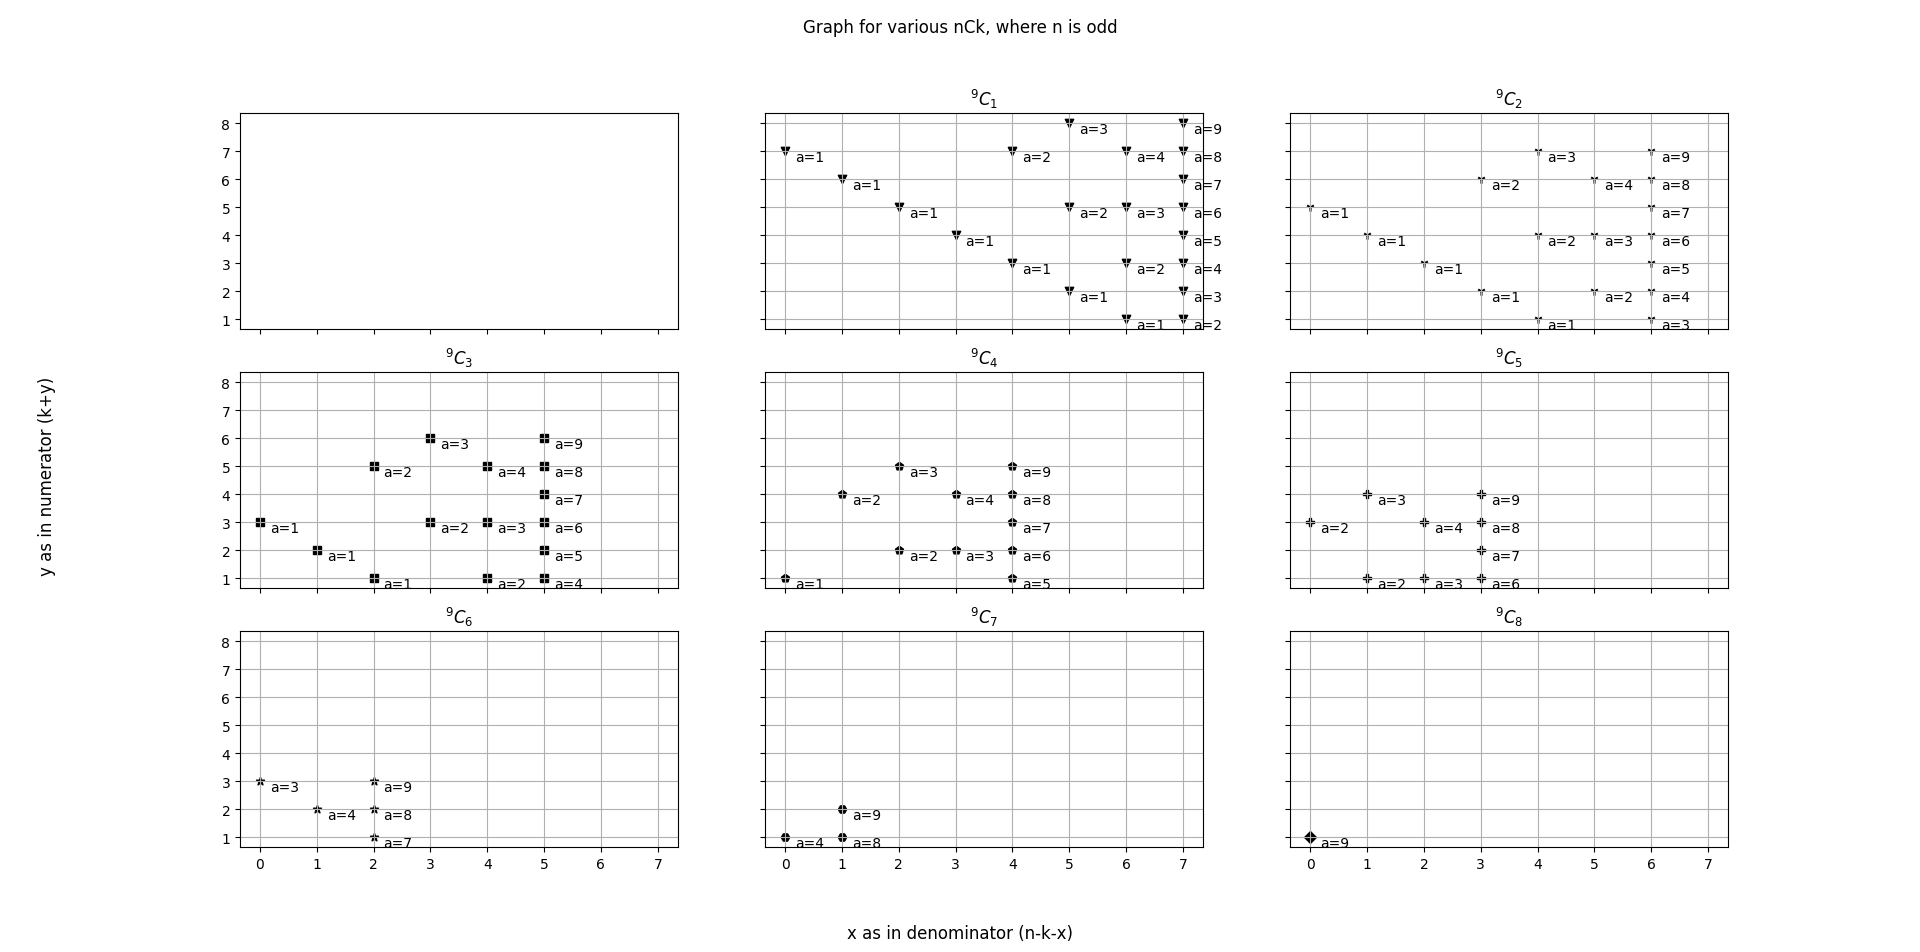
\includegraphics[width=\linewidth]{9Ck.png}
	\caption{Plot of $\Combination{9}{k}$}
	\label{9Ck}
\end{figure}
\begin{figure}[ph!]	
	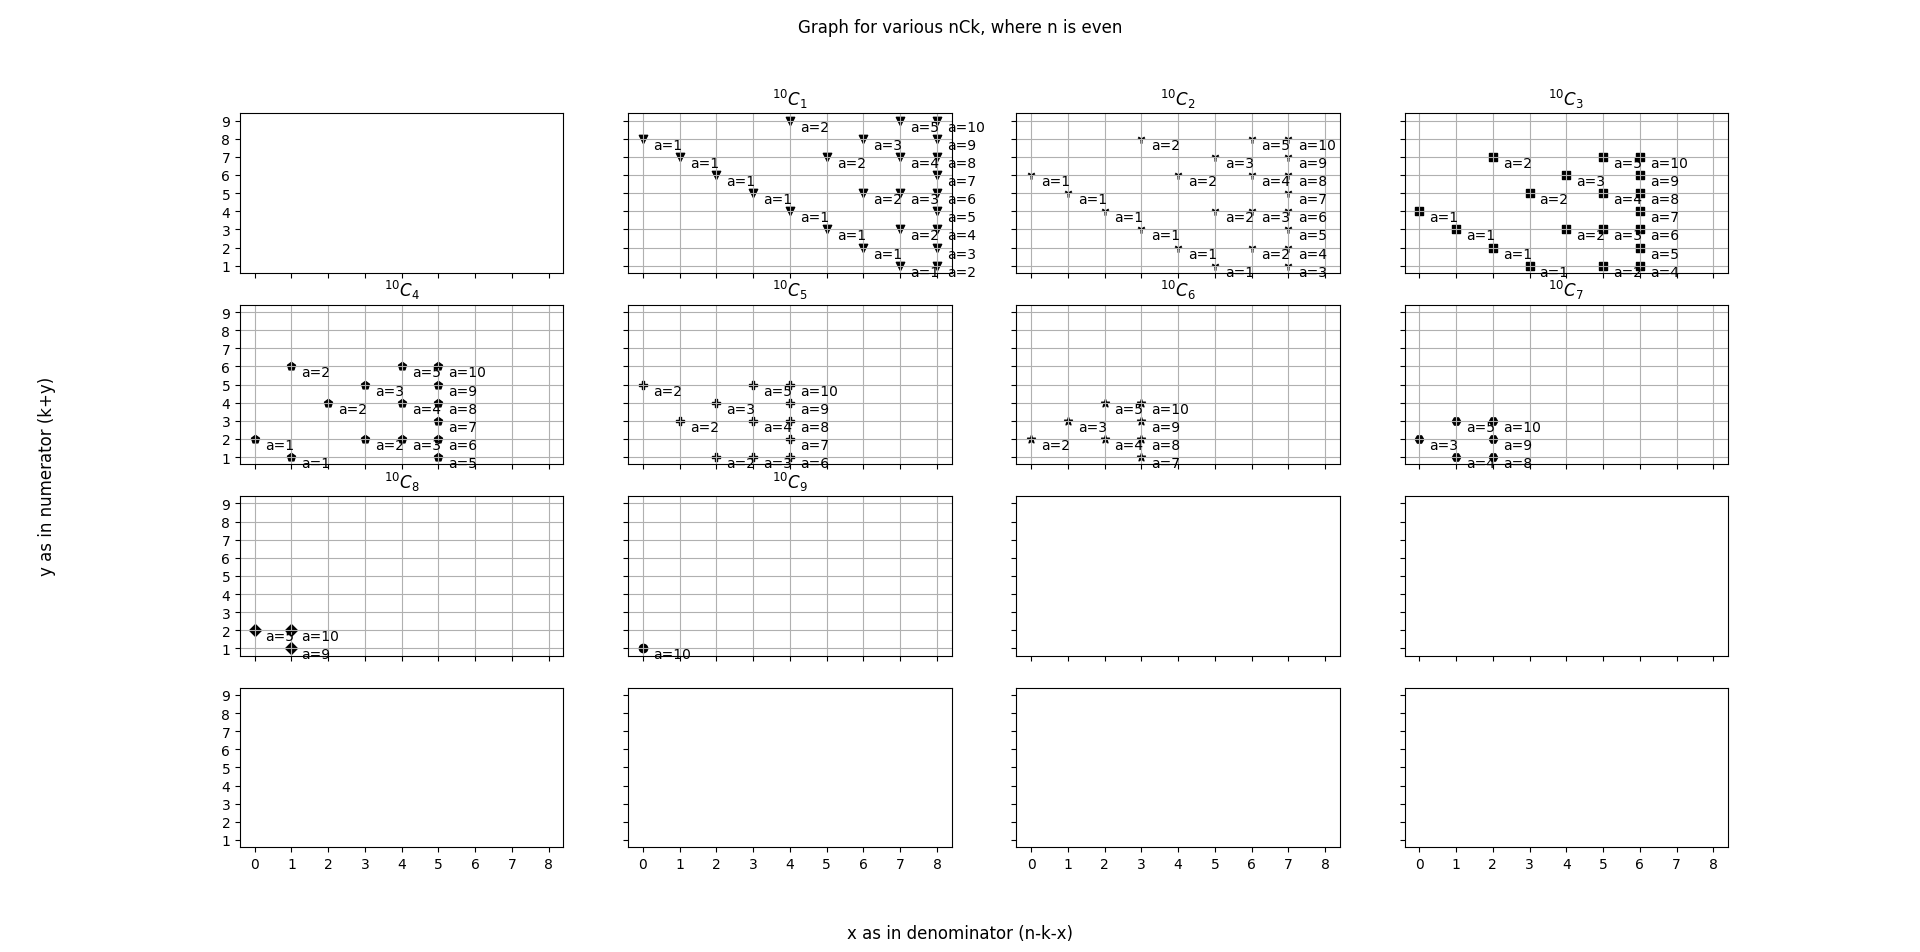
\includegraphics[width=\linewidth]{10Ck.png}
	\caption{Plot of $\Combination{10}{k}$}
	\label{10Ck}
\end{figure}	
\begin{figure}[ph!]	
	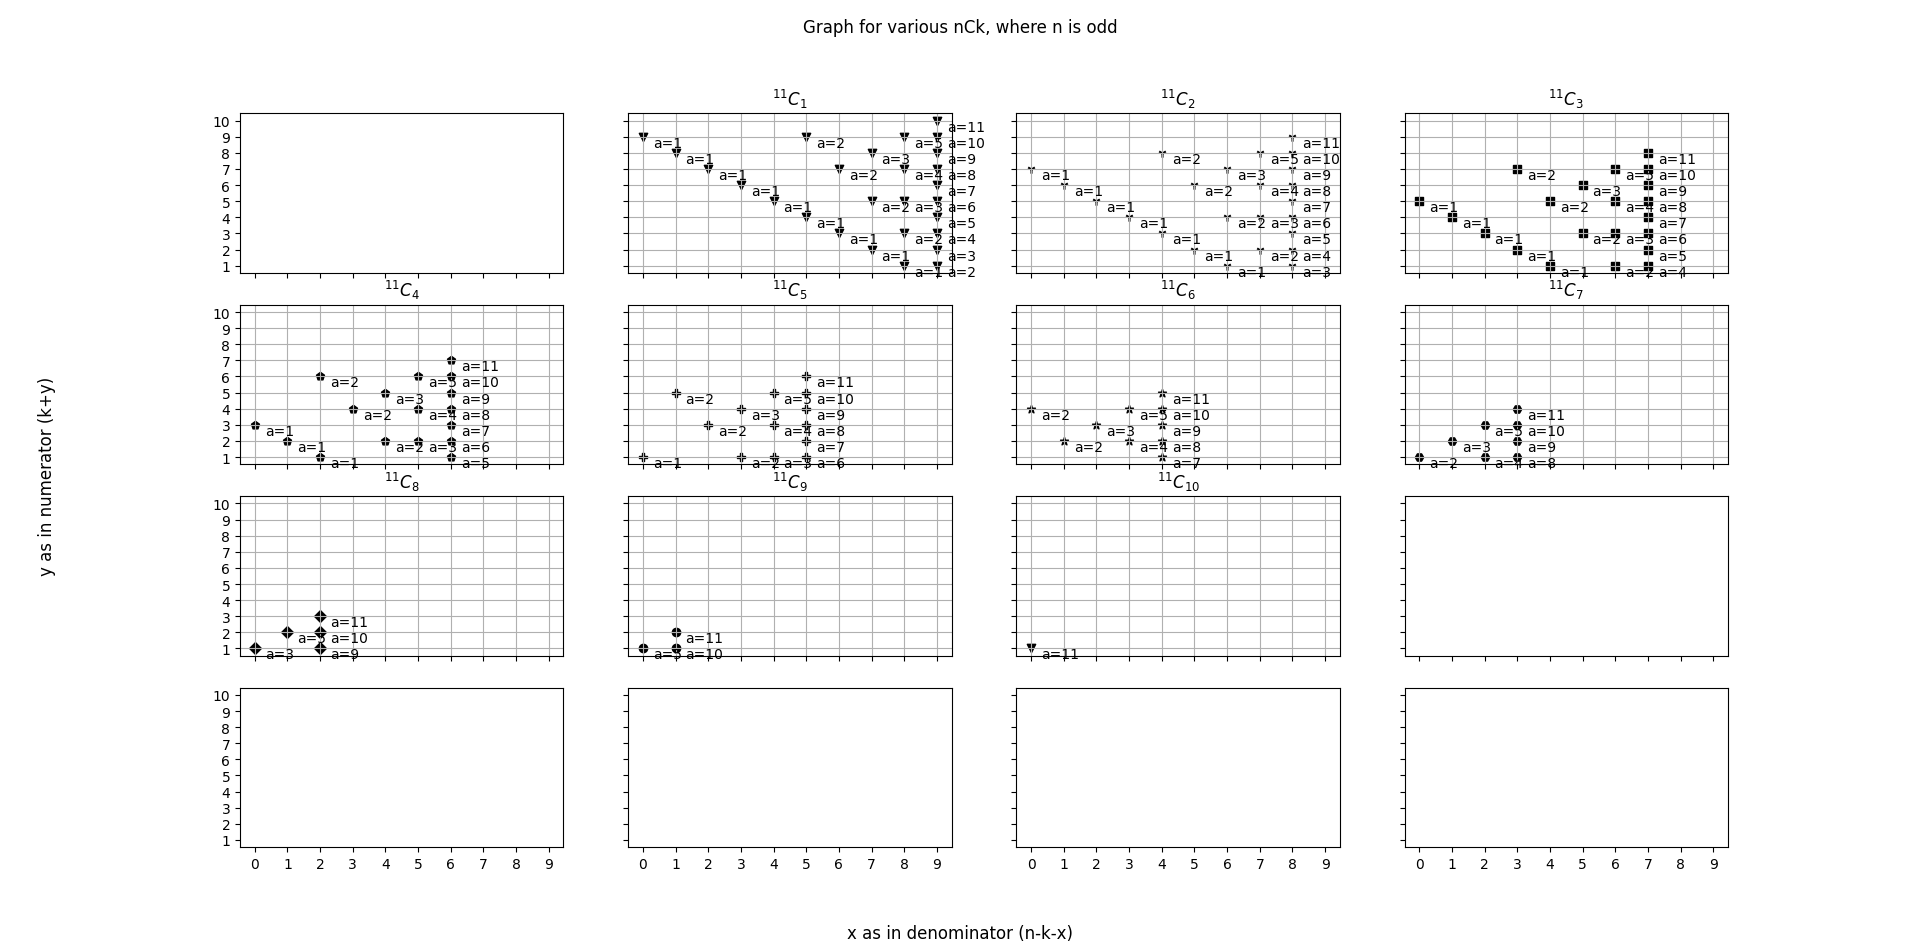
\includegraphics[width=\linewidth]{11Ck.png}
	\caption{Plot of $\Combination{11}{k}$}
	\label{11Ck}									
\end{figure}
\begin{figure}[ph!]	
	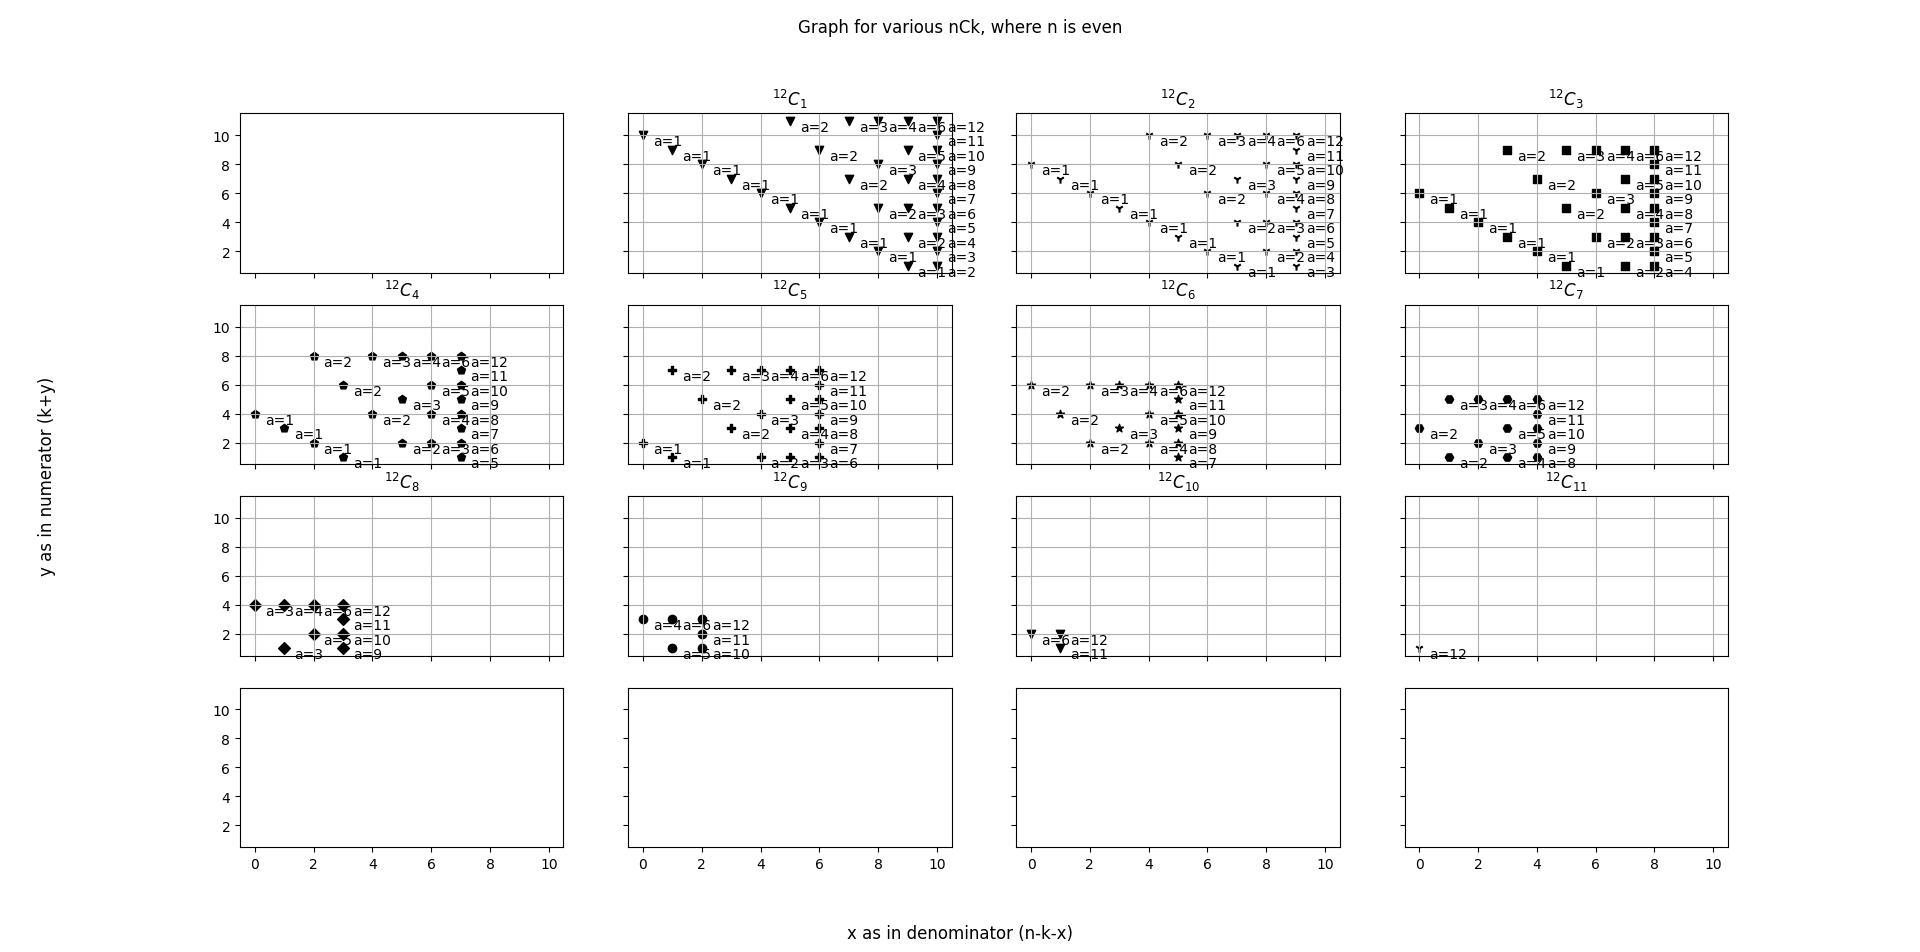
\includegraphics[width=\linewidth]{12Ck.png}
	\caption{Plot of $\Combination{12}{k}$}
	\label{12Ck}
\end{figure}	
\begin{figure}[ph!]	
	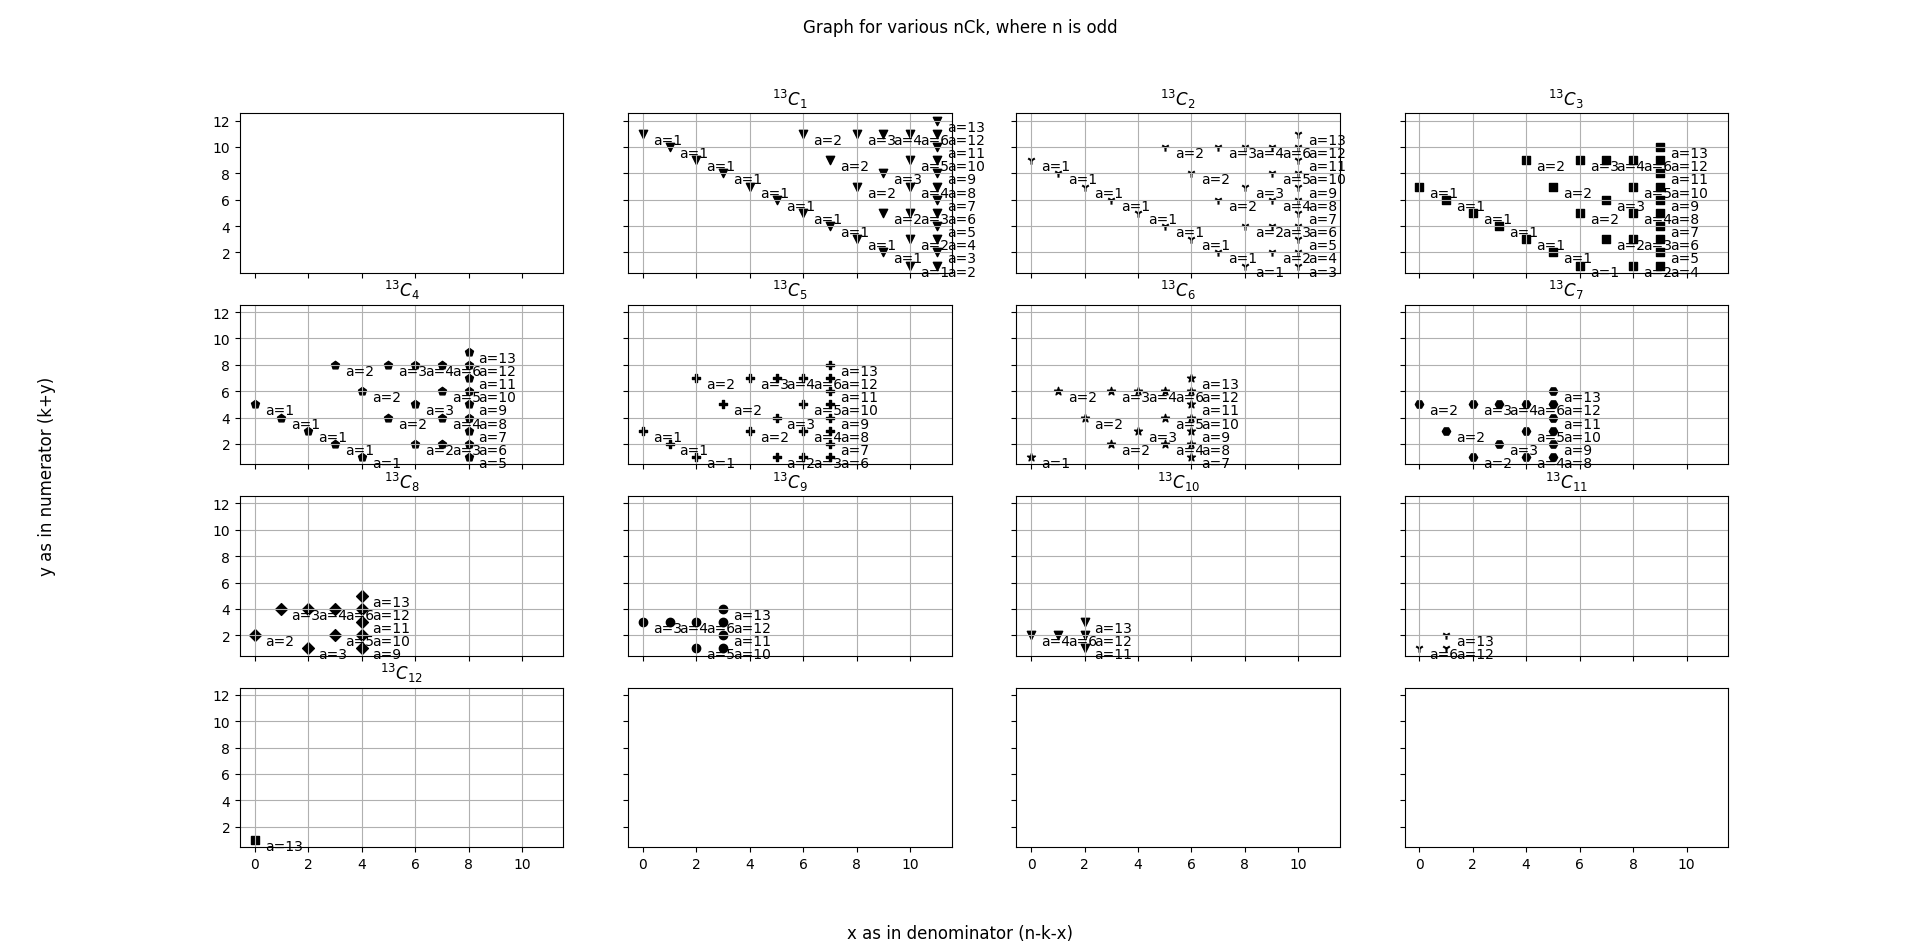
\includegraphics[width=\linewidth]{13Ck.png}
	\caption{Plot of $\Combination{13}{k}$}
	\label{13Ck}									
\end{figure}\newline
The code for these plots (Figure \ref{2Ck}-\ref{13Ck}) is given in appendix \ref{PythonCodeToGenerateGraph}.
\subsection{Delving deeper into the graphs}
Based on the images seen before it is clear that the values of $a$ for which an $x$ has a corresponding $y$ have a set of striking patterns if we analyze all $k$ combinations of $\Combination{n}{k}$ for a given $n$. 
\begin{enumerate}
	\item For a given $n$, graph is most dense for $\Combination{n}{1}$ and least dense for $\Combination{n}{n-1}$. In other words, maximum number of $a$ (and thus $x$ and $y$) points are present on the graph in the former case and least points are present on the graph in the later case.
	\item Vertical lines can be drawn for each $x$ (which goes into the denominator term $(n-k-x)$). 
	\item For $\Combination{n}{1}$, graph, the position of dots on the graph (a dot is a valid solution with a value of $a$), for any vertical line can be easily predicted. For the right most vertical line (equal to the value of $(n-\textbf{1}-1)$) for $x$, the dots start at the value of $2$ for the lowest value of $y=\textbf{1}$ and then keep incrementing by $1$ for every \textbf{$1$} position towards the top for a value of $(n-1)$ correspnding to the $y=(n-1)$. For the next left line (correspnding to the $(n-\textbf{2}-1)$), the dots start at the value of $1$ for the lowest value of $y=\textbf{2}$ and then keep incrementing at every \textbf{$2$} position by $1$. For the preceeding subsequent line at $(n-\textbf{3}-1)$, the dots start at the value of $1$ for the lowest value of $y=\textbf{3}$ and then keep incrementing at every \textbf{$3$} position. This pattern holds for every preceeding line. For a line at position $(n-\textbf{k}-1)$, the points start at the value of $1$ for the lowest value of $y=\textbf{k}$ and then keep incrementing at every \textbf{$k$} location by $1$.
	\item Horizontal lines can be drawn for each $y$ (which goes into the numerator term $(k+y)$).
	\item For $\Combination{n}{1}$, graph, the position of dots on the graph, for any horizontal line can be easily predicted. For a value of $y$ we consider $y+1$ and we find that the value of $a$ for the dots are nothing but the factors of $y+1$. Clearly prime numbers have no factors other than themselves and $1$.
	\item As we go towards higher $k$ (starting from $1$ and go towards $(n-1)$) for the $\Combination{n}{k}$, the $\Combination{n}{1}$ graph shifts digonally (left and downwards) and terms outside the boundaries of $ 1 \leq y \leq (n-k)$ and $0 \leq x \leq (n-k-1)$ keep 'falling off' the graph and 'disappear'. This we can call as the 'destruction picture' or 'low-to-high picture'. Please see the attached image at this URL \url{https://github.com/amit7urmc/CombinationsAndPrimes/blob/master/25_C_k_264.mp4}.
	\item As we go from higher to lower $k$ (starting from $(n-1)$ and towards 1) for the $\Combination{n}{k}$, the $\Combination{n}{1}$ graph shifts digonally (right and upwards) and terms within the boundaries of $ 1 \leq y \leq (n-k)$ and $0 \leq x \leq (n-k-1)$ keep 'joining' the graph and 'appear'. This we can call as the 'construction picture' or 'high-to-low picture'. Please see the attached image at this URL \url{https://github.com/amit7urmc/CombinationsAndPrimes/blob/master/25_C_k_reverse_264.mp4}.
	\item In either of the pictures (destruction or construction), we can pause at any $\Combination{n}{k}$ and we can calculate the value of combination as follows: All the numbers on the right most vertical lines go in the numerator and then in each vertical line highest point is taken as the divisor and its correspnding right most number as the dividend. The result of this goes into the numerator for each vertical line (except the right most line). e.g. for $\Combination{25}{19}$, we can pause the construction/destruction picture there (or straightaway calculate the state using the code given in the appendix \ref{PythonCodeToGenerateGraph}) and we see that the right most vertical line consists of $25, 24, 23, 22, 21 \text{ and } 20$. There are $5$ vertical lines (except the right most). For the first vertical line in the left, the highest vertical point is $a=4$ and its corresponding right most point is $a=24$. So the first vertical line 'collapses' to $24/4=6$. The subsequent line to the right 'collapses' to $25/5=5$ since the highest point is $a=5$ and its corresponding to the right most point $a=25$. Similarly we can get the remaining numbers as $24/6=4$, $24/8=3$ and $24/12=2$. All these $5$ numbers $(6,5,4,3 \text{ and } 2)$, go in the denominator and we get the answer as $\frac{25\times24\times23\times22\times21\times20}{6\times5\times4\times3\times2}=177100$, which is exactly what is the answer for $\Combination{25}{19}$. 
	\item In the light of these images and in the hindsight, it is easy to see now that prime numbers do not appear, on the number-line, at random afterall! There is a definite and simple rule governing their appearance on the number line. To simplify the discussion and summary consider this analogy: 
	\subitem In the beginning there is only one known prime in the list of primes i.e. [$2$] on the number line. 
	\subitem Now each number (in the list of primes so far) hops one step. If for any prime number (the number of steps) modulus (the prime number itself) is zero (i.e. it is an exact multiple of that prime), then we discard that number from consideration of prime. However if for all numbers (in the list of primes) there is some remainder on modulus, then that means this \textbf{new step or the new number} is not a multiple of any known prime.
	\subitem If in the above step we generate a prime then we add it to the list of known primes and the hopping continues until as long as desired. In the subsequent hops however this newly generated prime number 'joins' the hopping game.
	\subitem Thus it seems that in this hopping game, any new numbers is 'spared' if it is an exact multiple of any known prime. However if all known primes 'desert' that number then this 'new orphan' number sprouts and comes into existence and immediately joins the hopping game.
	\item To prove this computationally, we downloaded first known 1000 primes from \url{https://t5k.org/lists/small/1000.txt}  and compared it against the primes generated by this article's algorithm (in appendix \ref{PythonCodeToGeneratePrimes}). There is a perfect match!
	
\end{enumerate}
\begin{figure}[ph!]
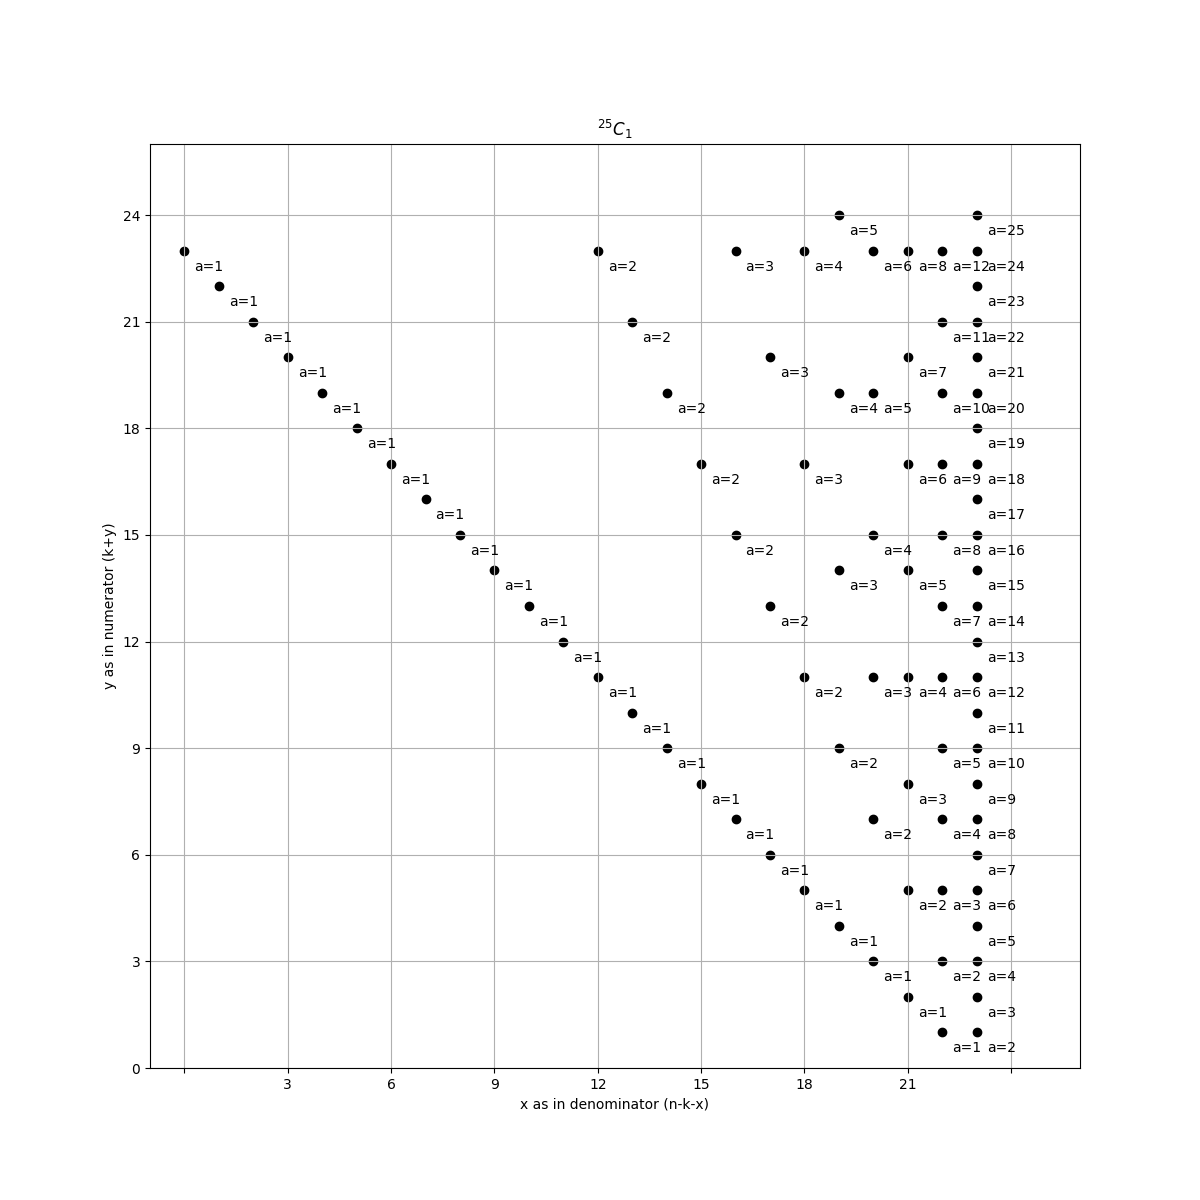
\includegraphics[width=\linewidth]{25_1_alone.png}
\caption{Distribution of $x,y \text{ and } a$ in the graph of $\Combination{25}{1}$}
\label{25_C_1_example}
\end{figure}
\begin{appendices}
	\section{Code to generate the plots as in \ref{Summary}}\label{PythonCodeToGenerateGraph}
	\begin{python}
from random import random
from math import ceil, sqrt, nan
import matplotlib.pyplot as plt 
from matplotlib.ticker import MaxNLocator

def create_chart_combination(n: int, k:int)->list[list[int], list[int], list[int]]:
    """
    Premise (See the accompanying PDF)
    -----------------------------------------------------------------------------
    | n     | k     | y                                                         |
    -----------------------------------------------------------------------------
    | Even  | n//2  | y = (a-1)\times n//2 - a\times x                          |
    | Even  | n//2-l| y = (a-1)\times n//2 + l \times (a+1) - a\times x         |
    | Even  | n//2+m| y = (a-1)\times n//2 - m \times (a+1) - a\times x         |
    | Odd   | n//2  | y = (a-1)\times n//2 + a - a\times x                      |
    | Odd   | n//2-l| y = (a-1)\times n//2 + a + l\times(a+1) - a\times x       |
    | Odd   | n//2+m| y = (a-1)\times n//2 + a -m\times(a+1) - a\times x        |
    -----------------------------------------------------------------------------
    The chart can be made in the following step.
    1. Decide n is even or odd.
    2. given k and n, decide if l or m is there and if yes what value.
    3. Get range of x such that 0 <= x <= (n-k-1)
    4. Solve for a(s) and y(s) for each x with restrain that 1 <= y <= (n-k).
    5. Return a list of three lists [x, y, a] # for plotting
    """
    IS_EVEN = n%2 == 0
    l, not_l_m, m = n//2-k if k < n//2 else None, n//2 if k==n//2 else None, k-n//2 if k > n//2 else None
    x = list(range(0,n-k,1))
    y = []
    solution_params = []    
    for each_x in x:
        a = []
        starting_guess = 1
        indiv_solution_params = []
        if IS_EVEN:
            if not_l_m:
                while True:
                    y_ = (starting_guess-1)*n//2 - (starting_guess*each_x)
                    if y_ > (2*(n//2)-k):
                        break                    
                    if y_ >= 1:
                        a.append(starting_guess)
                        indiv_solution_params.append((l,not_l_m,m,starting_guess))
                    starting_guess += 1
                y_s = list(map(lambda a_dash: (a_dash-1)*n//2 - (a_dash*each_x),a))
                y.append(y_s)
            elif l:
                while True:
                    y_ = (starting_guess-1)*(n//2) + l*(starting_guess+1) - (starting_guess*each_x)
                    if y_ > (2*(n//2)-k):
                        break
                    if y_ >= 1:
                        a.append(starting_guess)
                        indiv_solution_params.append((l,not_l_m,m,starting_guess))
                    starting_guess += 1
                y_s = list(map(lambda a_dash: (a_dash-1)*(n//2) +l*(a_dash+1) - (a_dash*each_x),a))
                y.append(y_s)    
            elif m:
                while True:
                    y_ = (starting_guess-1)*(n//2) -m*(starting_guess+1) - (starting_guess*each_x)
                    if y_ > (2*(n//2)-k):
                        break                    
                    if y_ >= 1:
                        a.append(starting_guess)
                        indiv_solution_params.append((l,not_l_m,m,starting_guess))
                    starting_guess += 1
                y_s = list(map(lambda a_dash: (a_dash-1)*(n//2) -m*(a_dash+1) - (a_dash*each_x),a))
                y.append(y_s)  
        else:
            if not_l_m:
                while True:
                    y_ = (starting_guess-1)*(n//2) +starting_guess - (starting_guess*each_x)
                    if y_ > ((2*(n//2)+1)-k):
                        break                    
                    if y_ >= 1:
                        a.append(starting_guess)
                        indiv_solution_params.append((l,not_l_m,m,starting_guess))
                    starting_guess += 1
                y_s = list(map(lambda a_dash: (a_dash-1)*(n//2)+a_dash - (a_dash*each_x),a))
                y.append(y_s)
            elif l:
                while True:
                    y_ = (starting_guess-1)*(n//2) +starting_guess + l*(starting_guess+1) - (starting_guess*each_x)
                    if y_ > ((2*(n//2)+1)-k):
                        break                    
                    if y_ >= 1:
                        a.append(starting_guess)
                        indiv_solution_params.append((l,not_l_m,m,starting_guess))
                    starting_guess += 1
                y_s = list(map(lambda a_dash: (a_dash-1)*(n//2)+a_dash +l*(a_dash+1) - (a_dash*each_x),a))
                y.append(y_s)    
            elif m:
                while True:
                    y_ = (starting_guess-1)*(n//2) +starting_guess -m*(starting_guess+1) - (starting_guess*each_x)
                    if y_ > ((2*(n//2)+1)-k):
                        break                    
                    if y_ >= 1:
                        a.append(starting_guess)
                        indiv_solution_params.append((l,not_l_m,m,starting_guess))
                    starting_guess += 1
                y_s = list(map(lambda a_dash: (a_dash-1)*(n//2)+a_dash -m*(a_dash+1) - (a_dash*each_x),a))
                y.append(y_s) 
        solution_params.append(indiv_solution_params)
    returned_x = []
    returned_y = []
    returned_params = []
    for each_y_list_index, each_y_list in enumerate(y):
        solution_params_ = solution_params[each_y_list_index]
        for each_y_index, each_y in enumerate(each_y_list):
            returned_x.append(x[each_y_list_index])
            returned_y.append(each_y)
            returned_params.append(solution_params_[each_y_index])
    returned_results = [returned_x, returned_y, returned_params]
    return returned_results

def create_one_case_graph(n: int, k: int)->None:
    max = n
    fig, ax = plt.subplots(nrows=1, ncols=1, figsize=(12,12))
    ax.set_xlim(right=n+1)
    ax.set_xlim(left=-1)
    ax.set_ylim(top=n+1)
    ax.set_ylim(bottom=0)
    ax.set_xticks(ticks=list(range(1,n-k,1)), labels=[str(i) for i in range(1,n-k,1)])
    ax.yaxis.set_major_locator(MaxNLocator(integer=True, min_n_ticks=1))
    ax.xaxis.set_major_locator(MaxNLocator(integer=True, min_n_ticks=1))
    x, y, params = create_chart_combination(n,k)
    ax.scatter(x=x, y=y, c=[[0,0,0]], marker='o')
    ax.grid(which='both')
    ax.set_title('$ ^{%d}C_{%d}$'%(n,k))
    for data_index, _ in enumerate(params):
        param = _
        annotation = f"a={param[3]}"
        xy = (x[data_index], y[data_index])
        ax.annotate(annotation, xy=xy, xytext=(10,-20),textcoords='offset pixels')
    ax.set_xlabel('x as in denominator (n-k-x)')
    ax.set_ylabel('y as in numerator (k+y)')
    fig.savefig(f'./{n}_{k}_alone.png')
    plt.close()

def create_all_cases_graph(n: list[int, int])->None:
    """
    Supplied one even and one add number. 0th index should be even while 1st index should be odd.
    """
    assert n[0]%2==0 and n[1]%2
    markers = ["o","v","1","s","p","P","*","H","D","X"]
    fig, axs1 = plt.subplots(nrows=int(ceil(sqrt(n[0]))),ncols=int(ceil(sqrt(n[0]))), sharey=True, sharex=True)
    for axs_row in axs1:
        for axs_col in axs_row:
            axs_col.yaxis.set_major_locator(MaxNLocator(integer=True, min_n_ticks=1))
            axs_col.xaxis.set_major_locator(MaxNLocator(integer=True, min_n_ticks=1))
    ## Draw for even numbers
    counter = 0
    for k in range(1,n[0],1):
        if(k%int(ceil(sqrt(n[0])))==0):
            counter += 1        
        x, y, params = create_chart_combination(n[0],k)
        axs1[counter][k%int(ceil(sqrt(n[0])))].scatter(x=x, y=y, c=[[0,0,0]], marker=markers[k%(len(markers)-1)])
        axs1[counter][k%int(ceil(sqrt(n[0])))].grid(which='both')
        axs1[counter][k%int(ceil(sqrt(n[0])))].set_title('$ ^{%d}C_{%d}$'%(n[0],k))
        for data_index, _ in enumerate(params):
            param = _
            annotation = f"a={param[3]}"
            xy = (x[data_index], y[data_index])
            axs1[counter][k%int(ceil(sqrt(n[0])))].annotate(annotation, xy=xy, xytext=(10,-10),textcoords='offset pixels')
    fig.suptitle("Graph for various nCk, where n is even")
    fig.supxlabel("x as in denominator (n-k-x)")
    fig.supylabel("y as in numerator (k+y)")
    
    fig, axs2 = plt.subplots(nrows=int(ceil(sqrt(n[1]))),ncols=int(ceil(sqrt(n[1]))), sharey=True, sharex=True)
    for axs_row in axs2:
        for axs_col in axs_row:
            axs_col.yaxis.set_major_locator(MaxNLocator(integer=True, min_n_ticks=1))
            axs_col.xaxis.set_major_locator(MaxNLocator(integer=True, min_n_ticks=1))    
    ## Draw for odd numbers
    counter = 0
    for k in range(1,n[1],1):
        if(k%int(ceil(sqrt(n[1])))==0):
            counter += 1        
        x, y, params = create_chart_combination(n[1],k)
        axs2[counter][k%int(ceil(sqrt(n[1])))].scatter(x=x, y=y, c=[[0,0,0]], marker=markers[k%(len(markers)-1)])
        axs2[counter][k%int(ceil(sqrt(n[1])))].grid(which='both')
        axs2[counter][k%int(ceil(sqrt(n[1])))].set_title('$ ^{%d}C_{%d}$'%(n[1],k))
        for data_index, _ in enumerate(params):
            param = _
            annotation = f"a={param[3]}"
            xy = (x[data_index], y[data_index]) 
            axs2[counter][k%int(ceil(sqrt(n[1])))].annotate(annotation, xy=xy, xytext=(10,-10),textcoords='offset pixels')       
    fig.suptitle("Graph for various nCk, where n is odd")
    fig.supxlabel("x as in denominator (n-k-x)")
    fig.supylabel("y as in numerator (k+y)")

    plt.show()        


                    
if __name__ == "__main__":
    create_all_cases_graph([2,3])
    create_all_cases_graph([4,5])
    create_all_cases_graph([6,7])
    create_all_cases_graph([8,9])
    create_all_cases_graph([10,11])  
    create_all_cases_graph([12,13])
    
    n=25
    for k in range(1,n,1):
        create_one_case_graph(n, k)      
	\end{python}
	\section{Code to generate the prime numbers as in \ref{Summary}}\label{PythonCodeToGeneratePrimes}
	\begin{python}
class generatePrime:

    def __init__(self, fileToWrite: str="./primeListGenerated.txt")-> None:
        self.primeNumbersDiscovered = [2]
        self.primeNumbersSteps = [0]
        self.runningNumber = 2
        self.primeNumbersDiscoveredListLength = 1
        self.fileToWrite = fileToWrite

    def yield_prime(self, upto_n:int)->None:
        with open(self.fileToWrite,"w") as fileHandle:
            fileHandle.write("primeNumbersGenerated\n")
            counter = 0
            while True:
                skipFlag = False
                self.runningNumber += 1
                for i in range(self.primeNumbersDiscoveredListLength):
                    self.primeNumbersSteps[i] += 1
                    if not self.runningNumber%self.primeNumbersDiscovered[i]:
                        skipFlag = True
                        break

                if not skipFlag:
                    self.primeNumbersDiscovered.append(self.runningNumber)
                    self.primeNumbersDiscoveredListLength += 1
                    self.primeNumbersSteps.append(0)
                    fileHandle.write(f"{self.runningNumber}\n")
                    counter += 1
                if counter > upto_n:
                    break
    
    def compare_against_known_result(self, know_result_file:str="./primeListGenerated.txt")->bool:
        present_absent = None
        with open(know_result_file, "r") as knownHandle, open(self.fileToWrite,"r") as calculateddHandle:
            knownResult = knownHandle.readlines()[1:]
            calculatedResult = calculateddHandle.readlines()[1:]
            assert len(knownResult) == len(calculatedResult)
            present_absent = [True if knownResult[i]==calculatedResult[i] else False for i in range(len(knownResult))]
        if all(present_absent):
            return True
        return False



if __name__ == "__main__":
    upto_n = 1000
    full_match_str = "full_match"
    some_mismatch_str = "some_mismatch"
    primeObj = generatePrime()
    primeObj.yield_prime(upto_n)
    full_match = primeObj.compare_against_known_result()
    print(f"We tried to match first known {upto_n} primes with those generated by this program. The answer is {full_match_str if full_match else some_mismatch_str}")
	
	\end{python}	
	This code is also available in github \url{https://github.com/amit7urmc/CombinationsAndPrimes}.
\end{appendices}
\end{document}